\section{Chapter~\ref{chapter:mvae}}
\label{sec:app:mvae}
\subsubsection{Dataset Descriptions}

\paragraph{MNIST/BinaryMNIST}
We use the MNIST hand-written digits dataset \cite{lecun1998gradient} with 50,000 examples for training, 10,000 validation, 10,000 testing. We also train on a binarized version to align with previous work \cite{larochelle2011neural}.
As in \cite{suzuki2016joint}, we use the Adam optimizer \cite{kingma2014adam} with a learning rate of 1e-3, a minibatch size of 100, 64 latent dimensions, and train for 500 epochs. We anneal $\beta$ from $0$ to $1$ linearly for the first 200 epochs. For the encoders and decoders, we use MLPs with 2 hidden layers of 512 nodes. We model $p(x_{1}|z)$ with a Bernoulli likelihood and $p(x_{2}|z)$ with a multinomial likelihood.

\paragraph{FashionMNIST}
This is an MNIST-like fashion dataset containing 28 x 28 grayscale images of clothing from 10 classes---skirts, shoes, t-shirts, etc \cite{xiao2017fashion}. We use identical hyperparameters as in MNIST. However, we employ a miniature DCGAN \cite{radford2015unsupervised} for the image encoder and decoder.

\paragraph{MultiMNIST}
This is variant of MNIST where between 0 and 4 digits are composed together on a 50x50 canvas. Unlike \cite{eslami2016attend}, the digits are fixed in location. We generate the text modality by concatenating the digit classes from top-left to bottom-right.
We use 100 latent dimensions, with the remaining hyperparameters as in MNIST. For the image encoder and decoder, we retool the DCGAN architecture from \cite{radford2015unsupervised}. For the text encoder, we use a bidirectional GRU with 200 hidden units. For the text decoder, we first define a vocabulary with ten digits, a start token, and stop token. Provided a start token, we feed it through a 2-layer GRU,  linear layers, and a softmax. We sample a new character and repeat until generating a stop token. We note that previous work has not explored RNN-VAE inference networks in multi-modal learning, which we show to work well with the MVAE.

\paragraph{CelebA}
The CelebFaces and Attributes (CelebA) dataset \cite{yang2015facial} contains over 200k images of celebrities. Each image is tagged with 40 attributes i.e. wears glasses, or has bangs. We use the aligned and cropped version with a selected 18 visually distinctive attributes, as done in \cite{perarnau2016invertible}. Images are rescaled to 64x64.
For the first experiment, we treat images as one modality, $x_{1}$, and attributes as a second modality, $x_{2}$ where a single inference network predicts all 18 attributes. We also explore a variation of MVAE, called MVAE19, where we treat each attribute as its own modality for a total of 19. To approximate the full objective, we set $k = 1$ for a total 21 ELBO terms.
We use Adam with a learning rate of $10^{-4}$, a minibatch size of 100, and anneal KL for the first 20 of 100 epochs. We again use DCGAN for image networks. For the attribute encoder and decoder, we use an MLP with 2 hidden layers of size 512. For MVAE19, we have 18 such encoders and decoders.

\subsubsection{Additional Results using the Joint Inference Network}

In the main paper, we reported marginal probabilities using $q(z|x_1)$ and showed that MVAE is state-of-the-art. Here we similarly compute marginal probabilities but using $q(z|x_1, x_2)$. Because importance sampling with either induced distribution yields an unbiased estimate, using a large number of samples should result in very similar log-likelihoods. Indeed, we find that the results do not differ much from the main paper: MVAE is still at the state-at-the-art.

\begin{table}[h!]
\centering
\small
\begin{tabular}{ l|c|c|c|c|c }
    \toprule
    Model & BinaryMNIST & MNIST & FashionMNIST & MultiMNIST & CelebA \\
    \hline
    \multicolumn{6}{c}{Estimating $\textup{log }p(x_{1})$ using $q(z|x_{1},x_{2})$} \\
    \hline
    JMVAE & -86.234 & -90.962 & \textbf{-232.401} & -153.026 & \textbf{-6234.542} \\
    MVAE & \textbf{-86.051} & \textbf{-90.616} & -232.539 & \textbf{-152.826} & -6237.104 \\
    MVAE19 & -- & -- & -- & -- & -6236.113 \\
    \hline
    \multicolumn{6}{c}{Estimating $\textup{log }p(x_{1},x_{2})$ using $q(z|x_{1},x_{2})$} \\
    \hline
    JMVAE & -86.304 & -91.031 & \textbf{-232.700} & \textbf{-153.320} & \textbf{-6238.280} \\
    MVAE & \textbf{-86.278} & \textbf{-90.851} & -233.007 & -153.478 & -6241.621 \\
    MVAE19 & -- & -- & -- & -- & -6239.957 \\
    \hline
    \multicolumn{6}{c}{Estimating $\textup{log }p(x_{1}|x_{2})$ using $q(z|x_{1},x_{2})$} \\
    \hline
    JMVAE & \textbf{-83.820} & \textbf{-88.436} & \textbf{-230.651} & \textbf{-145.761} & -6235.330 \\
    MVAE & -83.940 & -88.558 & -230.699 & -147.009 & -6235.368 \\
    MVAE19 & -- & -- & -- & -- & \textbf{-6233.330} \\
    \bottomrule
\end{tabular}
\caption{Similar estimates as in Table 2 (in main paper) but using $q(z|x_{1},x_{2})$ as an importance distribution (instead of $q(z|x_{1})$). Because VAE and CVAE do not have a multi-modal inference network, they are excluded.}
% \ndg{i don't think we really need this one?}}
\label{table:xy_results}
\end{table}

\begin{table}[h!]
\centering
\small
\begin{tabular}{ l|c|c|c|c|c }
    \toprule
    \multicolumn{6}{c}{Variance of Marginal Log Importance Weights: $\textup{var}(\textup{log}(\frac{p(x_1,z)}{q(z|x_1,x_2)}))$} \\
    \hline
    Model & BinaryMNIST & MNIST & FashionMNIST & MultiMNIST & CelebA \\
    \hline
    JMVAE & 22.387 & \textbf{24.962} & 28.443 & 35.822 & 80.808 \\
    MVAE & \textbf{21.791} & 25.741 & \textbf{18.092} & \textbf{16.437} & 73.871 \\
    MVAE19 & -- & -- & -- & -- & \textbf{71.546} \\
    \hline
    \multicolumn{6}{c}{Variance of Joint Log Importance Weights: $\textup{var}(\textup{log}(\frac{p(x_1,x_2,z)}{q(z|x_1,x_2)}))$} \\
    \hline
    JMVAE & 23.309 & 26.767 & 29.874 & 38.298 & 81.312 \\
    MVAE & \textbf{21.917} & \textbf{26.057} & \textbf{18.263} & \textbf{16.672} & 74.968 \\
    MVAE19 & -- & -- & -- & -- & \textbf{71.953} \\
    \hline
    \multicolumn{6}{c}{Variance of Conditional Log Importance Weights: $\textup{var}(\textup{log}(\frac{p(x_1,z|x_2)}{q(z|x_1,x_2)}))$} \\
    \hline
    JMVAE & 40.646 & 40.086 & 56.452 & 92.683 & 335.046 \\
    MVAE & \textbf{23.035} & \textbf{27.652} & \textbf{19.934} & \textbf{28.649} & 77.516 \\
    MVAE19 & -- & -- & -- & -- & \textbf{71.603} \\
    \bottomrule
\end{tabular}
\caption{Average variance of log importance weights for marginal, joint, and conditional distributions using $q(z|x_1,x_2)$.}
\label{table:xy_variances}
\end{table}

% For MVAE19 on CelebA, we can conduct a slightly different weak supervision experiment than the one shown in the paper: given a complete multi-modal example $(x_{1}, ..., x_{19})$, randomly keep $x_{i}$ with probability $p$ for each $i=1, ..., 19$. Doing so for all examples in the training set, we simulate the effect of missing modalities beyond the bi-modal setting. Here, the number of examples shown to the model is dependent on $p$ e.g. $p = 0.5$ suggests that on average, 1 out of every 2 $x_{i}$ are dropped. We vary $p$ from $0.001$ to $1$, train from scratch, and plot (1) the prediction accuracy per attribute and (2) the various data log-likelihoods. From Figure \ref{fig:dropout_prediction}, we conclude that the method is fairly robust to missing data. Even with $p=0.1$, we still see accuracy close to the prediction accuracy with full data.
% % \rdh{super cool!

\subsubsection{More on Weak Supervision}

In the main paper, we showed that we do not need that many complete examples to learn a good joint distribution with two modalities. Here, we explore the robustness of our model with missing data under more modalities. Using MVAE19 (19 modalities) on CelebA, we can conduct a different weak supervision experiment: given a complete multi-modal example $(x_{1}, ..., x_{19})$, randomly keep $x_{i}$ with probability $p$ for each $i=1, ..., 19$. Doing so for all examples in the training set, we simulate the effect of missing modalities beyond the bi-modal setting. Here, the number of examples shown to the model is dependent on $p$ e.g. $p = 0.5$ suggests that on average, 1 out of every 2 $x_{i}$ are dropped. We vary $p$ from $0.001$ to $1$, train from scratch, and plot (1) the prediction accuracy per attribute and (2) the various data log-likelihoods. From Figure \ref{fig:dropout_prediction}, we conclude that the method is fairly robust to missing data. Even with $p=0.1$, we still see accuracy close to the prediction accuracy with full data.

\begin{figure}[h!]
\centering
    \begin{subfigure}[b]{.24\linewidth}
        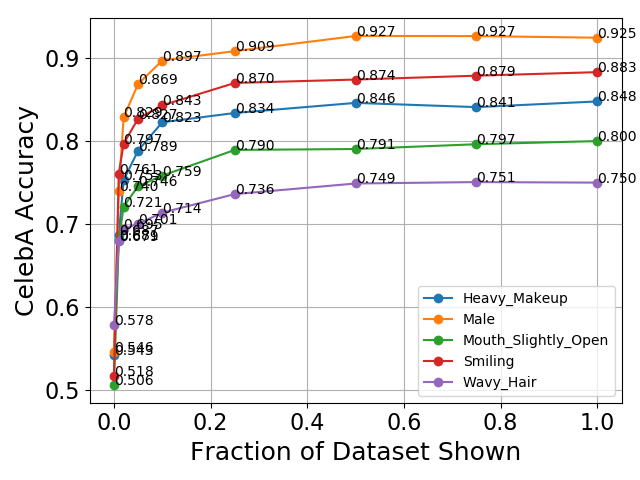
\includegraphics[width=\linewidth]{images/chapter3/weaksup/celeba19random}
        \caption{$p(y|x)$}
    \end{subfigure}
    \begin{subfigure}[b]{.24\linewidth}
        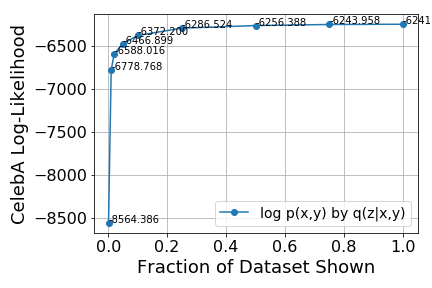
\includegraphics[width=\linewidth]{images/chapter3/weaksup/celeba19joint}
        \caption{$\textup{log }p(x,y)$}
    \end{subfigure}
    \begin{subfigure}[b]{.24\linewidth}
        \includegraphics[width=\linewidth]{images/chapter3/weaksup/celeba19marginal}
        \caption{$\textup{log }p(x)$}
    \end{subfigure}
    \begin{subfigure}[b]{.24\linewidth}
        \includegraphics[width=\linewidth]{images/chapter3/weaksup/celeba19conditional}
        \caption{$\textup{log }p(x|y)$}
    \end{subfigure}
    \caption{We randomly drop input features $x_{i}$ with probability $p$. Figure (a) shows the effect of increasing $p$ from $0.001$ to $1$ on the  accuracy of sampling the correct attribute given an image. Figure (b) and (c) show changes in log marginal and log conditional approximations as $p$ increases. In all cases, we see close-to-best performance using only 10\% of the complete data.}
    % \ndg{fix x label (not dropout \%)}
    \label{fig:dropout_prediction}
\end{figure}

\subsubsection{Table of Weak Supervision Results}

In the main text, we showed a series of plots detailing the performance the MVAE on a weak supervision task. Here we provide additional tables.

\begin{table}
\centering
\scriptsize
\begin{tabular}{ l|c|c|c|c|c|c|c|c|c }
    \toprule
    Model & 0.1\% & 0.2\% & 0.5\% & 1\% & 2\% & 5\% & 10\% & 50\% & 100\% \\
    \hline
    AE & 0.4143 & 0.5429 & 0.6448 & 0.788 & 0.8519 & 0.9124 & 0.9269 & 0.9423 & 0.9369 \\
    NN & 0.6618 & 0.6964 & 0.7971 & 0.8499 & 0.8838 & 0.9235 & 0.9455 & 0.9806 & 0.9857 \\
    LOGREG & 0.6565 & 0.7014 & 0.7907 & 0.8391 & 0.8510 & 0.8713 & 0.8665 & 0.9217 & 0.9255 \\
    RBM & 0.7152 & 0.7496 & 0.8288 & 0.8614 & 0.8946 & 0.917 & 0.9257 & 0.9365 & 0.9379 \\
    VAE & 0.2547 & 0.284 & 0.4026 & 0.6369 & 0.8016 & 0.8717 & 0.8989 & 0.9183 & 0.9311 \\
    JMVAE & 0.2342 & 0.2809 & 0.3386 & 0.6116 & 0.7869 & 0.8638 & 0.9051 & 0.9498 & 0.9572 \\
    MVAE & 0.2842 & 0.6254 & 0.8593 &0.8838 & 0.9394 & 0.9584 & 0.9711 & 0.9678 & 0.9681 \\
    \bottomrule
\end{tabular}
\caption{Performance on MNIST with a fraction of paired examples. Here we compute the accuracy (out of 1) of predicting the correct digit in each image.}
\label{table:x_results}
\end{table}

\begin{table}
\centering
\scriptsize
\begin{tabular}{ l|c|c|c|c|c|c|c|c|c }
    \toprule
    Model & 0.1\% & 0.2\% & 0.5\% & 1\% & 2\% & 5\% & 10\% & 50\% & 100\% \\
    \hline
    NN & 0.6755 & 0.701 & 0.7654 & 0.7944 & 0.8102 & 0.8439 & 0.862 & 0.8998 & 0.9318 \\
    LOGREG & 0.6612 & 0.7005 & 0.7624 & 0.7627 & 0.7728 & 0.7802 & 0.8015 & 0.8377 & 0.8412 \\
    RBM & 0.6708 & 0.7214 & 0.7628 & 0.7690 & 0.7805 & 0.7943 & 0.8021 & 0.8088 & 0.8115 \\
    VAE & 0.5316 & 0.6502 & 0.7221 & 0.7324 & 0.7576 & 0.7697 & 0.7765 & 0.7914 & 0.8311 \\
    JMVAE & 0.5284 & 0.5737 & 0.6641 & 0.6996 & 0.7437 & 0.7937 & 0.8212 & 0.8514 & 0.8828 \\
    MVAE & 0.4548 & 0.5189 & 0.7619 & 0.8619 & 0.9201 & 0.9243 & 0.9239 & 0.9478 & 0.947 \\
    \bottomrule
\end{tabular}
\caption{Performance on FashionMNIST with a fraction of paired examples. Here we compute the accuracy of predicting the correct class of attire in each image.}
\label{table:x_results}
\end{table}

\begin{table}[tb]
\centering
\scriptsize
\begin{tabular}{ l|c|c|c|c|c|c|c|c|c }
    \toprule
    Model & 0.1\% & 0.2\% & 0.5\% & 1\% & 2\% & 5\% & 10\% & 50\% & 100\% \\
    \hline
    JMVAE & 0.0603 & 0.0603 & 0.0888 & 0.1531 & 0.1699 & 0.1772 & 0.4765 & 0.4962 & 0.4955 \\
    MVAE & 0.09363 & 0.1189 & 0.1098 & 0.2287 & 0.3805 & 0.4289 & 0.4999 & 0.5121 & 0.5288 \\
    \bottomrule
\end{tabular}
\caption{Performance of several models on MultiMNIST with a fraction of paired examples. Here compute the average accuracy of predicting each digit correct (by decomposing the string into individual digits, at most 4).}
\label{table:x_results}
\end{table}

\subsubsection{Details on Weak Supervision Baselines}

The VAE used the same image encoder as the MVAE. JMVAE used identical architectures as the MVAE with a hyperparameter $\alpha = 0.01$. The RBM has a single layer with 128 hidden nodes and is trained using contrastive divergence. NN uses the image encoder and label/string decoder as in MVAE, thereby being a fair comparison to supervised learning. For MNIST, we trained each model for 500 epochs. For FashionMNIST and MultiMNIST, we trained each model for 100 epochs. All other hyperparameters were kept constant between models.

\subsubsection{More of the effects of sampling more ELBO terms}

In the main paper, we stated that with higher $k$ (sampling more ELBO terms), we see a steady decrease in variance. This drop in variance can be attributed to two factors: (1) additional un-correlated randomness from sampling more when reparametrizing for each ELBO \cite{burda2015importance}, or (2) additional ELBO terms to better approximate the intractable objective. Figure~\ref{fig:mtest} (c) shows that the variance still drops consistently when using a fixed $\epsilon \sim N(0, 1)$ for computing all ELBO terms, indicating independent contributions of additional ELBO terms and randomness.

\begin{figure}[h!]
\centering
    \begin{subfigure}[b]{.32\linewidth}
        \centering
        \includegraphics[width=\linewidth]{images/chapter3/mtest/joint_proba.pdf}
        \caption{}
        \label{fig:mtest:joint}
    \end{subfigure}
    \begin{subfigure}[b]{.32\linewidth}
        \centering
        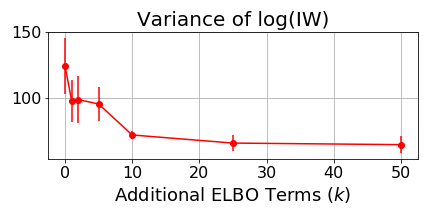
\includegraphics[width=\linewidth]{images/chapter3/mtest/variance.pdf}
        \caption{}
        \label{fig:mtest:var}
    \end{subfigure}
    \begin{subfigure}[b]{.32\linewidth}
        \centering
        \includegraphics[width=\linewidth]{images/chapter3/mtest/variance-fixed-epsilon.pdf}
        \caption{}
        \label{fig:mtest:var:epsilon}
    \end{subfigure}
    \caption{Effect of approximating the MVAE objective with more ELBO terms on (a) the joint log-likelihood and (b) the variance of the log importance weights over 3 independent runs. Similarly, (c) compute the variance but fixes a single $\epsilon \sim N(0, 1)$ when reparametrizing for each ELBO. (b) and (c) imply that switching from $k=0$ to $k=1$ greatly reduces the variance in the importance distribution defined by the inference network(s).}
    \label{fig:mtest}
\end{figure}

\subsubsection{More on the Computer Vision Transformations}

We copy Figure 4 in the main paper but show more samples and increase the size of each image for visibility. The MVAE is able to learn all 6 transformations jointly under the PoE inference network.

\begin{figure}[h!]
    \centering
    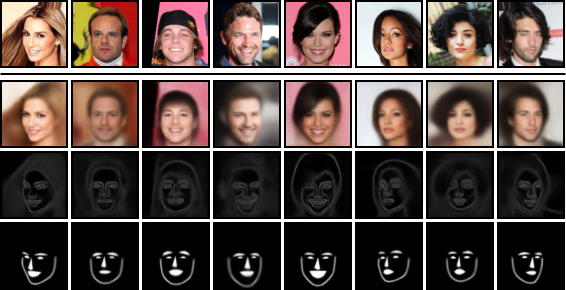
\includegraphics[width=\linewidth]{images/chapter3/vision/recon_edge_face}
    \caption{\textit{Edge Detection and Facial Landscapes}: The top row shows 8 ground truth images randomly chosen from the CelebA dataset. The second to fourth rows respectively plot the reconstructed image, edge, and facial landscape masks using the trained MVAE decoders and  $q(z|x_{1}, ..., x_{6})$.}
    \label{fig:vision_recon}
\end{figure}

\begin{figure}[h!]
    \centering
    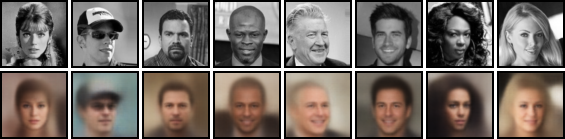
\includegraphics[width=\linewidth]{images/chapter3/vision/colorization}
    \caption{\textit{Colorization}: The top row shows ground truth grayscale images. The bottom row show reconstructed color images.}
    \label{fig:vision_color}
\end{figure}

\begin{figure}[h!]
    \centering
    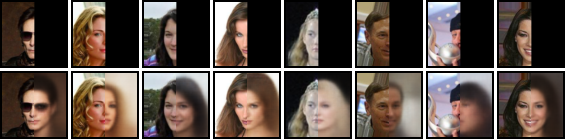
\includegraphics[width=\linewidth]{images/chapter3/vision/fill_in_blank}
    \caption{\textit{Fill in the Blank}: The top row shows ground truth CelebA images with half of each image obscured. The bottom row replaces the obscured part with a reconstruction.}
    \label{fig:vision_blank}
\end{figure}

\begin{figure}[h!]
    \centering
    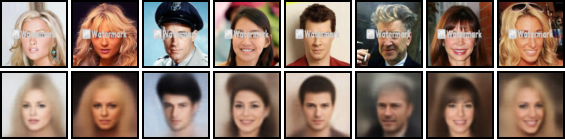
\includegraphics[width=\linewidth]{images/chapter3/vision/watermark}
    \caption{\textit{Removing Watermarks}: The top row shows ground truth CelebA images, each with an added watermark. The bottom row shows the reconstructed image with the watermark removed.}
    \label{fig:vision_watermark}
\end{figure}

\subsubsection{More on Machine Translation}

We provide more samples on (1) sampling joint (English, Vietnamese) pairs of sentences from the prior $N(0,1)$, (2) translating English to Vietnamese by sampling from $p(x_{\textup{en}}|z)$ where $z \sim q(z|x_{\textup{vi}})$, and (3) translating Vietnamese to English by sampling from $p(x_{\textup{vi}}|z)$ where $z \sim q(z|x_{\textup{en}})$. 

\begin{table}
\centering
\scriptsize
\begin{tabular}{ l|l }
  \toprule
  \textbf{Type} & \textbf{Sentence} \\
  \hline
  $x_{\textup{en}} \sim p(x_{\textup{en}}|z=z_0)$ & it's a problem . \\
  $x_{\textup{vi}} \sim p(x_{\textup{vi}}|z=z_0)$ & \foreignlanguage{vietnamese}{nó là một công việc .} \\
  $\textsc{GoogleTranslate}(x_{\textup{vi}})$ & it is a job . \\
  \hline
  $x_{\textup{en}} \sim p(x_{\textup{en}}|z=z_0)$ & we have an idea . \\
  $x_{\textup{vi}} \sim p(x_{\textup{vi}}|z=z_0)$ & \foreignlanguage{vietnamese}{chúng tôi có thể làm được .} \\
  $\textsc{GoogleTranslate}(x_{\textup{vi}})$ & we can do it . \\
  \hline
  $x_{\textup{en}} \sim p(x_{\textup{en}}|z=z_0)$ & And as you can see , this is a very powerful effect of word of mouth . \\
  $x_{\textup{vi}} \sim p(x_{\textup{vi}}|z=z_0)$ & \foreignlanguage{vietnamese}{và một trong những điều này đã xảy ra với những người khác , và chúng} \\
  & \foreignlanguage{vietnamese}{tôi đã có một số người trong số các bạn đã từng nghe về những điều này .} \\
  $\textsc{GoogleTranslate}(x_{\textup{vi}})$ & and one of these has happened to other people, and we've had \\
  & some of you guys already heard about this . \\
  \hline
  $x_{\textup{en}} \sim p(x_{\textup{en}}|z=z_0)$ & this is a photograph of my life . \\
  $x_{\textup{vi}} \sim p(x_{\textup{vi}}|z=z_0)$ & \foreignlanguage{vietnamese}{Đây là một bức ảnh .} \\
  $\textsc{GoogleTranslate}(x_{\textup{vi}})$ & this is a photo . \\
  \hline
  $x_{\textup{en}} \sim p(x_{\textup{en}}|z=z_0)$ & thank you . \\
  $x_{\textup{vi}} \sim p(x_{\textup{vi}}|z=z_0)$ & \foreignlanguage{vietnamese}{xin cảm ơn .} \\
  $\textsc{GoogleTranslate}(x_{\textup{vi}})$ & thank you . \\
  \hline
  $x_{\textup{en}} \sim p(x_{\textup{en}}|z=z_0)$ & i'm not kidding . \\
  $x_{\textup{vi}} \sim p(x_{\textup{vi}}|z=z_0)$ & \foreignlanguage{vietnamese}{tôi không nói đùa .} \\
  $\textsc{GoogleTranslate}(x_{\textup{vi}})$ & i am not joking . \\
  \bottomrule
\end{tabular}
\caption{Examples of ``paired" reconstructions from a single sample $z_0 \sim q(z|x_{\textup{en}}, x_{\textup{vi}})$. Many of the translations are not exact but instead capture a close interpretation of the true meaning. The MVAE performs better on shorter sentences.}
\label{table:translation_examples}
\end{table}

\begin{table}
\centering
\scriptsize
\begin{tabular}{ l|l }
  \toprule
  \textbf{Type} & \textbf{Sentence} \\
  \hline
  $x_{\textup{en}} \sim p_{\textup{data}}$ & this was one of the highest points in my life. \\
  $x_{\textup{vi}} \sim p(x_{\textup{vi}}|z(x_{\textup{en}}))$ & \foreignlanguage{vietnamese}{Đó là một gian tôi vời của cuộc đời tôi.} \\
  $\textsc{GoogleTranslate}(x_{\textup{vi}})$ & It was a great time of my life. \\
  \hline
  $x_{\textup{en}} \sim p_{\textup{data}}$ & i am on this stage . \\
  $x_{\textup{vi}} \sim p(x_{\textup{vi}}|z(x_{\textup{en}}))$ & \foreignlanguage{vietnamese}{tôi đi trên sân khấu .} \\
  $\textsc{GoogleTranslate}(x_{\textup{vi}})$ & me on stage .\\
  \hline
  $x_{\textup{en}} \sim p_{\textup{data}}$ & do you know what love is ? \\
  $x_{\textup{vi}} \sim p(x_{\textup{vi}}|z(x_{\textup{en}}))$ & \foreignlanguage{vietnamese}{Đó yêu của những ?} \\
  $\textsc{GoogleTranslate}(x_{\textup{vi}})$ & that's love ?\\
  \hline
  $x_{\textup{en}} \sim p_{\textup{data}}$ & today i am 22 . \\
  $x_{\textup{vi}} \sim p(x_{\textup{vi}}|z(x_{\textup{en}}))$ & \foreignlanguage{vietnamese}{hãy nay tôi sẽ tuổi .} \\
  $\textsc{GoogleTranslate}(x_{\textup{vi}})$ & I will be old now . \\
  \hline
  $x_{\textup{en}} \sim p_{\textup{data}}$ & so i had an idea . \\
  $x_{\textup{vi}} \sim p(x_{\textup{vi}}|z(x_{\textup{en}}))$ & \foreignlanguage{vietnamese}{tôi thế tôi có có thể vài tưởng tuyệt .} \\
  $\textsc{GoogleTranslate}(x_{\textup{vi}})$ & I can have some good ideas . \\
  \hline
  $x_{\textup{en}} \sim p_{\textup{data}}$ & the project's also made a big difference in the lives of the <unk> . \\
  $x_{\textup{vi}} \sim p(x_{\textup{vi}}|z(x_{\textup{en}}))$ & \foreignlanguage{vietnamese}{tôi án này được ra một Điều lớn lao cuộc sống của chúng người} \\
  & \foreignlanguage{vietnamese}{sống chữa hưởng .} \\
  $\textsc{GoogleTranslate}(x_{\textup{vi}})$ & this project is a great thing for the lives of people who live and thrive . \\
  \bottomrule
\end{tabular}
\caption{Examples of Vietnamese MVAE translations of English sentences. We use Google translate to re-translate back to English.}
\end{table}

\begin{table}[tb]
\centering
\scriptsize
\begin{tabular}{ l|l }
  \toprule
  \textbf{Type} & \textbf{Sentence} \\
  \hline
  $x_{\textup{vi}} \sim p_{\textup{data}}$ & \foreignlanguage{vietnamese}{Đó là thời điểm tuyệt vọng nhất trong cuộc đời tôi .} \\
  $x_{\textup{en}} \sim p(x_{\textup{en}}|z(x_{\textup{vi}}))$ & this is the most bad of the life . \\
  $\textsc{GoogleTranslate}(x_{\textup{vi}})$ & it was the most desperate time in my life . \\
  \hline
  $x_{\textup{vi}} \sim p_{\textup{data}}$ & \foreignlanguage{vietnamese}{cảm ơn .} \\
  $x_{\textup{en}} \sim p(x_{\textup{en}}|z(x_{\textup{vi}}))$ & thank . \\
  $\textsc{GoogleTranslate}(x_{\textup{vi}})$ & thank you . \\
  \hline
  $x_{\textup{vi}} \sim p_{\textup{data}}$ & \foreignlanguage{vietnamese}{trước tiên , tại sao chúng lại có ấn tượng xấu như vậy ?} \\
  $x_{\textup{en}} \sim p(x_{\textup{en}}|z(x_{\textup{vi}}))$ & first of all, you do not a good job ? \\
  $\textsc{GoogleTranslate}(x_{\textup{vi}})$ & First, why are they so bad? \\
  \hline
  $x_{\textup{vi}} \sim p_{\textup{data}}$ & \foreignlanguage{vietnamese}{Ông ngoại của tôi là một người thật đáng <unk> phục vào thời ấy .} \\
  $x_{\textup{en}} \sim p(x_{\textup{en}}|z(x_{\textup{vi}}))$ & grandfather is the best experience of me family . \\
  $\textsc{GoogleTranslate}(x_{\textup{vi}})$ & My grandfather was a worthy person at the time . \\
  \hline
  $x_{\textup{vi}} \sim p_{\textup{data}}$ & \foreignlanguage{vietnamese}{Đứa trẻ này 8 tuổi .} \\
  $x_{\textup{en}} \sim p(x_{\textup{en}}|z(x_{\textup{vi}}))$ & this is man is 8 years old . \\
  $\textsc{GoogleTranslate}(x_{\textup{vi}})$ & this child is 8 years old . \\
  \bottomrule
\end{tabular}
\caption{Rxamples of English MVAE translations of Vietnamese sentences. We use Google translate to translate to English as a ground truth.}
\end{table}

\section{Chapter~\ref{chapter:antivae}}

\subsubsection{Description of Datasets}

We provide details in preprocessing for datasets used in the experiments in the main text. In total, we tested AntiVAE on seven datasets: static MNIST, dynamic MNIST, FashionMNIST, OMNIGLOT, Caltech 101 Silhouettes, Frey Faces, and Histopathology patches. As in previous literature, static MNIST uses a fixed binarization of images whereas dynamic MNIST resamples images from the training dataset at each minibatch. In dynamic MNIST, the validation and test sets have fixed binarization. We do an identical dynamic resampling procedure for OMNIGLOT. Caltech101 is given as binary data, so we cannot resample at training time, which we find to cause overfitting on the test set. For grayscale images that cannot be binarized, we would like to parameterize the generative model as a Gaussian distribution. In practice, we found this choice to cause over-prioritization of the reconstruction term, essentially causing the VAE to behave like a regular autoencoder. Instead, we find that a logistic distribution over the 256 grayscale domain avoids this failure mode. We use the default variance constraints as in \cite{tomczak2017vae}. We now provide a brief description to introduce each dataset.

\paragraph{MNIST} is a dataset of hand-written digits from 0 to 9 split into 60,000 examples for training and 10,000 for testing. We use 10,000 randomly chosen images from the training set as a validation group.

\paragraph{FashionMNIST} Similar to MNIST, this more difficult dataset contains 28x28 \textit{grayscale} images of 10 different articles of clothing e.g. skirts, shoes, shirts, etc. The sizing and splits are identical to MNIST.

\paragraph{OMNIGLOT} is a dataset with 1,623 hand-wrriten characters from 50 different alphabets. Unlike the MNIST family of datasets, each character is only represented by 20 images, making this dataset more difficult. The training set is 24,345 examples with 8,070 test images. We again take 10\% of the training data as validation.

\paragraph{Caltech 101 Silhouettes} contains silhouettes of 101 different object classes in black and white: each image has a filled polygon on a white background. There are 4,100 training images, 2,264 validation datapoints and 2,307 test examples. Like OMNIGLOT, this task is difficult due to the limited data set.

\paragraph{FreyFaces} is a collection of portrait photos of one individual with varying emotional expressions for a total of 2,000 images. We use 1,565 for training, 200 validation, and 200 test examples.

\paragraph{Histopathology Patches} is a dataset from ten different biopsies of patients with cancer (e.g. lymphona, leukemia) or anemia. The dataset is originally in color with 336 x 448 pixel images. The data was processed to be 28 x 28 grayscale. The images are split in 6,800 training, 2,000 validation, and 2,000 test images. We refer to \cite{tomczak2016improving} for exact details.

\subsubsection{Evaluation Details} To compute the test log-likelihood (in any of the experiments), we use $k=100$ samples to estimate the following:

\begin{equation}
    \log \mathbf{E}_{z \sim q_\phi(z|x)}[\frac{p_\theta(x, z)}{q_\phi(z|x)}] \approx \log \frac{1}{k}\sum_{i=1}^{k}[\frac{p_\theta(x, z)}{q_\phi(z|x)}]
    \label{eqn:marginal}
\end{equation}
where $q_\phi(z|x)$ is an amortized inference network, $p_\theta(x|z)$ is a generative model, and $p(z)$ is a simple prior. We use (unbiased) i.i.d. samples to estimate Equation~\ref{eqn:marginal}. The final number reported is the average test log likelihood on the test set.

\subsubsection{Convolutional Architectures}
In the main text, we present results where $q_\phi(z|x)$ and $p_\theta(x|z)$ are parameterized by feedforward neural networks (multilayer perceptrons). While that architecture choice was made for simplicitly, we recognize that modern encoder/decoders have evolved beyond linear layers. Thus, we ran a subset of the experiments using DCGAN architectures \cite{radford2015unsupervised}. Specifically, we design $q_\phi(z|x)$ using 3 convolutional layers and $p_\theta(x|z)$ with 3 deconvolutional layers and 1 convolutional layer.

\begin{table}
\scriptsize
\centering
\begin{tabular}{r|ccccccc}
    Model & stat. MNIST & dyn. MNIST & FashionMNIST & Omniglot & Caltech  & Hist. \\
    \toprule
    VAE & -90.58 & -90.02 & -2767.97 & -108.97 & -116.15 &  -3218.16\\
    AntiVAE & -90.25 & -89.53 & -2762.02 & -108.40 & -115.14 & -3213.83 \\
    VAE+IWAE & -89.19 & -88.61 & -2758.72 & -107.52 & -116.25 & -3213.05 \\
    AntiVAE+IWAE & -89.01 & -88.13 & -2751.11 & -107.44 & -115.04 & -3209.98 \\
\end{tabular}
\caption{Test log likelihoods between the VAE and AntiVAE using (de)convolutional architectures for encoders and decoders. All images were reshaped to 32 by 32 to match standard DCGAN input sizes. }
\label{table:results_conv}
\end{table}

Table~\ref{table:results_conv} shows log-likelihoods on a test set for a variety of image datasets. Like experiments presented in the main text, we find improvements in density estimation when using antithetics. This agrees with our intuition that more representative samples benefit learning regardless of architecture choice.

\subsubsection{Variance over Independent Runs}
In the main text, we report the average test log likelihoods over 5 runs, each with a different random seed. Here, we report in Table~\ref{table:error} the variance as well (which we could not fit in the main table).

\begin{table}
\tiny
\centering
\begin{tabular}{r|cccccc}
    Dataset & VAE & AntiVAE & VAE+IWAE & AntiVAE+IWAE & VAE+10-NF & AntiVAE+10-NF \\
    \toprule
    StaticMNIST & $-90.44 \pm 0.031$ & $-89.74 \pm 0.066$ & $-89.78 \pm 0.080$ & $-89.71 \pm 0.059$ & $-90.07 \pm 0.033$ & $-89.77 \pm 0.042$ \\
    DynamicMNIST & $-86.96 \pm 1.398$ & $-86.94 \pm 1.412$ & $-86.71 \pm 1.778$ & $-86.62 \pm 1.426$ & $-86.93 \pm 1.132$ & $-86.57 \pm 1.173$ \\
    FashionMNIST & $-2819.13 \pm 1.769$ & $-2807.06 \pm 1.591$ & $-2797.02 \pm 1.714$ & $-2793.01 \pm 1.174$ & $-2803.98 \pm 1.487$ & $-2801.90 \pm 1.459$ \\
    Omniglot & $-110.65 \pm 0.141$ & $-110.13 \pm 0.063$ & $-109.32 \pm 0.134$ & $-109.48 \pm 0.104$ & $-110.03 \pm 0.178$ & $-109.43 \pm 0.057$ \\
    Caltech101 & $-127.26 \pm 0.254$ & $-124.87 \pm 0.213$ & $-123.99 \pm 0.262$ & $-123.35 \pm 0.195$ & $128.62 \pm 0.278$ & $-126.72 \pm 0.247$ \\
    FreyFaces & $-1778.78 \pm 4.649$ & $-1758.66 \pm 7.581$ & $-1772.06 \pm 7.275$ & $-1771.47 \pm 5.783$ & $-1780.61 \pm 4.595$ & $-1777.26 \pm 6.467$ \\
    Histopathology & $-3320.37 \pm 6.136$ & $-3294.23 \pm 1.543$ & $-3311.23 \pm 2.859$ & $-3305.91 \pm 1.972$ & $-3328.68 \pm 5.426$ & $-3303.00 \pm 1.517$ \\
    \end{tabular}
\caption{Identical to Table 1 in the main text but we include an errorbar over 5 runs. We find the differences induced by antithetics to be significant.}
\label{table:error}
\end{table}

\subsubsection{Runtime Experiments}
To measure runtime, we compute the average wall-time of the forward and backward pass over a single epoch with fixed hyperparameters for VAE and AntiVAE. Namely, we use a minibatch size of 128 and vary the number of samples $k=8, 16$. The measurements are in seconds using a Titan X GPU with CUDA 9.0. The implementation of the forward pass in PyTorch is vectorized across samples for both VAE and AntiVAE. Thus the comparison of runtime should be fair. We report the results in the Table.~\ref{table:runtime}.

\begin{table}
\tiny
\centering
\begin{tabular}{r|r|ccccccc}
    $k$ & Model & StaticMNIST & DynamicMNIST & FashionMNIST & OMNIGLOT & Caltech101  & FreyFaces & Hist. Patches \\
    \toprule
    8 & VAE & $0.0132 \pm 0.011$ & $0.0122 \pm 0.010$ & $0.0142 \pm 0.009$ & $0.0144 \pm 0.015$ & $0.0188 \pm 0.034$ & $0.0283 \pm 0.052$ & $0.0173 \pm 0.028$ \\
    8 & AntiVAE & $0.0179 \pm 0.011$ & $0.0156 \pm 0.009$ & $0.0173 \pm 0.010$ & $0.0164 \pm 0.017$ & $0.0220 \pm 0.036$ & $0.0334 \pm 0.054$ & $0.0196 \pm 0.029$ \\
    8 & AntiVAE (Cheng) & $0.0242 \pm 0.014$ & $0.0210 \pm 0.010$ & $0.0231 \pm 0.009$ & $0.0221 \pm 0.015$ & $0.0353 \pm 0.040$ & $0.040 \pm 0.062$ & $0.0303 \pm 0.026$\\
    \hline
    16 & VAE & $0.0228 \pm 0.009$ & $0.0182 \pm 0.011$ & $0.0207 \pm 0.010$ & $0.0181 \pm 0.015$ & $0.0275 \pm 0.035$ & $0.0351 \pm 0.049$ & $0.0245 \pm 0.027$\\
    16 & AntiVAE & $0.0252 \pm 0.009$ & $0.0240 \pm 0.011$ & $0.0288 \pm 0.010$ & $0.0256 \pm 0.015$ & $0.0308 \pm 0.035$ & $0.0384 \pm 0.049$ & $0.0315 \pm 0.027$ \\
    16 & AntiVAE (Cheng) & $0.0388 \pm 0.011$ & $0.0396 \pm 0.010$ & $0.0452 \pm 0.011$ & $0.0399 \pm 0.015$ & $0.0461 \pm 0.038$ & $0.0550 \pm 0.054$ & $0.0505 \pm 0.033$ \\
\end{tabular}
\caption{A comparison of runtime estimates between VAE and AntiVAE over different datasets. The number reported is the number of seconds for 1 forward and backward pass of a minibatch of size 128.}
\label{table:runtime}
\end{table}

To compute the additional cost of antithetic sampling, we divided the average runtimes of AntiVAE by the average runtimes of VAE and took the mean, resulting in 22.8\% increase in running time (about 0.004 seconds). We note that AntiVAE (Cheng) is more expensive due to vectorizing Helmert's transformation.

\subsubsection{Importance of Differentiability}
We report the numbers plotted in Figure4e, which showed that differentiability in antithetic sampling is the driving force behind sample diversity. The numbers reported are averaged over 5 runs on Histopathology.

\begin{table}
\small
\centering
\begin{tabular}{l|ccc}
    Epoch & VAE & AntiVAE (no backprop) & AntiVAE (with backprop) \\
    \toprule
    1 & $0.302 \pm  0.031$ & $0.301 \pm 0.026$ & $0.479 \pm 0.021$\\
    10 & $0.102 \pm 0.008$ & $0.103 \pm 0.022$ & $0.348 \pm 0.024$ \\
    20 & $0.068 \pm 0.006$ & $0.065 \pm 0.010$ &  $0.143 \pm 0.016$ \\
    50 & $0.040 \pm 0.005$ & $0.033 \pm 0.006$ & $0.063 \pm 0.004$ \\
    100 & $0.030 \pm 0.002$ & $0.028 \pm 0.008$ & $0.042 \pm 0.009$ \\
\end{tabular}
\caption{Variance of the first $k/2$ samples (non-antithetics) as measured over five independent runs on Histopathology. Without backprop, the variance is roughly equivalent to regular VAE.}
\label{table:diff_study}
\end{table}

As an aside, it is important to check that by adding differentiability, we do not introduce any unintended effects. For example, one might ask if differentiability leads to collapse of the VAE to a deterministic autoencoder (AE), thereby learning to ``sample" only the mean. To confirm that this is not the case, we measure the average variance (across dimensions and examples in the test set) of the variational posterior $q(z|x)$ when trained as a VAE versus as a AntiVAE.

\begin{table}
\small
\centering
\begin{tabular}{l|cc}
    Dataset & VAE & AntiVAE \\
    \toprule
    StaticMNIST & 0.253 & 0.290 \\
    DynamicMNIST & 0.269 & 0.290 \\
    FashionMNIST & 0.049 & 0.049 \\
    OMNIGLOT & 0.208 & 0.285\\
    Caltech101 & 0.179 & 0.182\\
    FreyFaces & 0.048 & 0.061\\
    Histopathology & 0.029 & 0.028\\
\end{tabular}
\caption{Learned variance of the approximate Gaussian posterior with and without antithetics. We measure variance on a variety of datasets.}
\label{table:collapse_study}
\end{table}

If differentiating through antithetic sampling led to ignoring noise, we would expect $q(z|x)$ to be deterministic i.e. near 0 variance. This does not appear to be the case, as shown in Table~\ref{table:collapse_study}.


\subsubsection{Deriving One-Liner Transformations}

We provide a step-by-step derivation for $g(\cdot)$ in one-liner transformations, namely from Gaussian to Cauchy and Exponential. We skip Log Normal as its formulation from a Gaussian variate is trivial. Below, let $X$ represent a normal variate and let $Y$ be a random variable in the desired distribution family.

\paragraph{Exponential} Let $F(X) = 1 - \exp^{-\lambda X}$. Parameters: $\lambda$. We start with $F(F^{-1}(Y)) = Y$.
\begin{align*}
    1 - \exp^{-(\lambda F^{-1}(Y))} &= Y \\
    \exp^{-(\lambda F^{-1}(Y))} &= 1 - Y \\
    -(\lambda F^{-1}(Y)) &= \log (1 - Y) \\
   \lambda F^{-1}(Y) &= -\log (1 - Y) \\
   F^{-1}(Y)& = -\frac{1}{\lambda} \log (1 - Y) \\
\end{align*}
Since $1 - Y \in \text{U}(0, 1)$ and $Y \in \text{U}(0, 1)$, we can replace $1 - Y$ with $Y$.
Then $F^{-1}(Y) = -\frac{1}{\lambda}\log Y$.

\paragraph{Cauchy}
Let $F(X) = \frac{1}{2} + \frac{1}{\pi}\arctan(\frac{X - x_0}{\gamma})$. Parameters: $x_0$, $\gamma$.
\begin{align*}
    \frac{1}{2} +   \frac{1}{\pi}\arctan(\frac{F^{-1}(Y) - x_0}{\gamma}) &= Y \\
    \arctan(\frac{F^{-1}(Y) - x_0}{\gamma}) &= \pi(Y - \frac{1}{2}) \\
    F^{-1}(Y) &= \gamma(\tan(\pi(Y - \frac{1}{2})) + x_0) \\
    F^{-1}(Y) &= \gamma(\tan(\pi Y) + x_0) \\
\end{align*}
In practice, we only optimize over $\gamma$, fixing $x_0$ to be 0.

\subsubsection{Deriving Antithetic Hawkins-Wixley}

We provide the following derivation for computing an antithetic $\chi^2$ variate using a normal approximation to the $\chi^2$ distribution. We assume the reader is familiar with the inverse CDF transform (as reviewed in the main text). \cite{hawkins1986note} presented the following fourth root approximation of a $\chi^2_n$ variate, denoted $X^{(1)}$ with $n$ degrees of freedom as distributed according to the following Gaussian:
\begin{equation}
    (X^{(1)}/n)^{1/4} \sim N(1 - \frac{3}{16n} - \frac{7}{512n^2} + \frac{231}{8192n^3}, \frac{1}{8n} + \frac{3}{128n^2} - \frac{23}{1024n^3})
\end{equation}
We can separately define a unit Gaussian variate, $Z^{(1)} \sim N(0, 1)$ such that
\begin{equation}
    Z^{(1)} = ((X^{(1)}/n)^{1/4} - (1 - \frac{3}{16n} - \frac{7}{512n^2} + \frac{231}{8192n^3})) \cdot \frac{1}{\sqrt{\frac{1}{8n} + \frac{3}{128n^2} - \frac{23}{1024n^3}}}
\end{equation}
Notice this is just the standard reparameterization trick reversed \cite{rezende2014stochastic}.
Independently, we can define a second $\chi^2_n$ variate, $X^{(2)}$ and unit Gaussian variate $Z^{(2)}$ in the same manner.
\begin{equation}
    Z^{(2)} = ((X^{(2)}/n)^{1/4} - (1 - \frac{3}{16n} - \frac{7}{512n^2} + \frac{231}{8192n^3})) \cdot \frac{1}{\sqrt{\frac{1}{8n} + \frac{3}{128n^2} - \frac{23}{1024n^3}}}
\end{equation}
As each $Z$ is distributed as $N(0, 1)$, the inverse CDF transform amounts to:
\begin{equation}
    Z^{(2)} = -Z^{(1)}
\end{equation}

Expanding each $Z$, we can derive a closed form solution:
\begin{align*}
    \small
    % ((X^{(2)}/n)^{1/4} - (1 - \frac{3}{16n} - \frac{7}{512n^2} + \frac{231}{8192n^3})) &= ((X^{(1)}/n)^{1/4} - (1 - \frac{3}{16n} - \frac{7}{512n^2} + \frac{231}{8192n^3})) \\
    (X^{(2)}/n)^{1/4} &= 2(1 - \frac{3}{16n} - \frac{7}{512n^2} + \frac{231}{8192n^3})) - (X^{(1)}/n)^{1/4} \\
    X^{(2)} &= n[2(1 - \frac{3}{16n} - \frac{7}{512n^2} + \frac{231}{8192n^3})) - (X^{(1)}/n)^{1/4}]^4
\end{align*}

This is the approximation we use in the main text. Coincidentally, \cite{wilson1931distribution} present a similar approximation but as a third root that is more popular. In the main text, we noted that we could not use this as it led negative antithetic variances. To see why, we first write their approximation:

\begin{equation}
    (X^{(1)}/n)^{1/3} \sim N(1 - \frac{2}{9n}, \frac{2}{9n})
\end{equation}

We end with the following antithetic Wilson-Hilferty equation:

\begin{equation}
    X^{(2)} = n\left[2(1 - \frac{2}{9n}) - (x^{(1)}/n)^{1/3}\right]^3
\end{equation}

The issue lies in the cube root. If $(x^{(1)}/n)^{1/3} \geq 2(1 - \frac{2}{9n})$, then inference is ill-posed as a Normal distribution with 0 or negative variance does not exist.

\subsubsection{Cheng's Solution to the Constrained Sampling Problem}
\label{sec:methods}

In the main text, we frequently reference a second algorithm, other than \cite{marsaglia1980c69} to solve the constrained sampling problem. Here we walk through the derivation of \cite{cheng1984generation,pullin1979generation} (which we present results for in the main text):

We first review a few useful characteristics of Gamma variables, then review an important transformation with desirable properties, and finally apply it to draw representative samples from a Gaussian distribution.

\paragraph{Invariance of Scaling Gamma Variates}

We wish to show that Gamma random variables are closed under scaling by a constant and under normalization by independent Gamma variates.

\begin{lem} If $x \sim \textup{Gamma}(\mu, \alpha)$ where $\mu > 0$ represents shape and $\alpha > 0$ represents rate, and $y = cx$ for some constant $c \in \mathbf{R}^{+}$, $y \sim \textup{Gamma}(\mu, \frac{\alpha}{c})$.
\label{lemma:mul_gamma}
\end{lem}
\begin{proof}
In generality, let the chain rule be $f_y(y) = F_x(g^{-1}(y))|\frac{dx}{dy}|$ where $f$ is the cumulative distribution function for a random variable. Applying this to a Gamma: $F_y(y) = \frac{\alpha^{\mu}(y/k)^{\mu-1} \exp^{-\alpha y/k}}{\Gamma(\mu)} = \frac{(\alpha /k)^{\mu}Y^{\mu-1}\exp^{-y\cdot \alpha/k}}{\Gamma(\mu)} = \textup{Gamma}(\mu, \frac{\alpha}{k})$.
\end{proof}

\begin{lem} Let $x_1, x_2, ..., x_k$ be $\textup{Gamma}(\mu, \alpha)$ variates and let $x_{k+1}$ be a $\textup{Gamma}(k\mu, \alpha)$ variate independent of $x_i$, for $i = 1, ..., k$. Then, $y_i = x_{k+1}(\frac{x_i}{\sum_{j=1}^{k} x_j})$ where $y_i \sim \textup{Gamma}(\mu, \alpha)$.
\label{lemma:many_gamma}
\end{lem}
\begin{proof} See \cite{aitchison1963inverse}.
\end{proof}
% \s{where is this used?}

% \ndg{this is a lemma not a def?}
\begin{lem} If $x \sim N(0, 1)$, then $x^2 \sim \chi^2_1$. Additionally, $x^2 \sim \textup{Gamma}(\frac{1}{2}, \frac{1}{2})$.
\label{lemma:normal_chi}
\end{lem}
\begin{proof} By definition.
\end{proof}

\begin{corollary} If $x \sim N(0, \sigma^2)$, then $\frac{x^2}{\sigma^2} \sim \chi^2_1$. Furthermore, we can say $x^2 \sim \sigma^2 \chi^2_1 = \sigma^2 \cdot \textup{Gamma}(\frac{1}{2}, \frac{1}{2}) = \textup{Gamma}(\frac{1}{2}, \frac{1}{2\sigma^2})$.
\label{corollary:normal_gamma}
\end{corollary}

\begin{proof} Direct application of Lemma~\ref{lemma:mul_gamma},~\ref{lemma:normal_chi}.
\end{proof}

\paragraph{Helmert's Transformation}

Given a random sample of size $k$ from any Gaussian distribution, Helmert's transformation \cite{helmert1875berechnung,pegoraro2012transformation} allows us to get $k-1$ new i.i.d. samples normally distributed with zero mean and the same variance as the original distribution: Let $x_1, ..., x_k \sim N(\mu, \sigma^2)$ be $k$ i.i.d. samples. We define the Helmert transformed variables, $y_2, ..., y_k$ as:

\begin{equation}
    y_j = \frac{\sum_{i=j}^{k} x_i - (k + 1 - j) x_{j-1}}{[(k + 1 - j)(k + 2 - j)]^{1/2}}
\label{eqn:helmert}
\end{equation}

for $j = 2, ..., k$. Helmert's transformation guarantees that for new samples:
\begin{prop}
    $y_2, ..., y_k$ are independently distributed according to $N(0, \sigma^2)$ such that $\sum_{i=2}^{k} y_i^2 = \sum_{i=1}^{k}(x_i - \bar{x})^2$ where $\bar{x} = \frac{1}{k}\sum_{i=1}^{k} x_i$.
\label{prop:helmert}
\end{prop}
\begin{proof} See \cite{helmert1875berechnung} or \cite{kruskal1946helmert}.
\end{proof}

Critically, Prop.~\ref{prop:helmert} also informs us that (1) the sample variance of $y_2, ..., y_k$ is equal to the sample variance of $x_1, ..., x_k$, and (2) $y_i, i=2,...,k$ can be chosen independently of $\bar{x}$. These properties will be important in the next subsection.

\paragraph{Choosing Representative Samples}

% \s{i think it would be good to end the previous section with the text you have in the intro:. more samples help, but how to pick them? i.i.d vs. something else. then transition into cheng}
% \ndg{+1}

% \s{pseudocode is great, but had a very hard time reading this section. consider rewriting.}
% \ndg{i found this section hard to follow... try SE's suggestions and then i'll read again. try to only say what is needed for your algorithm, and to keep telling us why you are doing each step...}
% \mwu{rewrote!}

We are tasked with the following problem: we wish to generate $k$ i.i.d. samples $x_1, ..., x_k \sim N(\mu, \sigma^2)$ subject to the following constraints:
\begin{align}
    \frac{1}{k}\sum_{i=1}^{k} x_i = \bar{x} &= \eta \label{eqn:constraint1}\\
    \frac{1}{k}\sum_{i=1}^{k}(x_i - \bar{x})^2 = s^2 &= \delta^2 \label{eqn:constraint2}
\end{align}
where by definition $\bar{x} \sim N(\mu, \frac{\sigma^2}{k})$ and $(k-1)s^2 / \sigma^2 \sim \chi^2_{k-1}$. We assume that $\eta$ and $(k-1)\delta^2/\sigma^2$ are particular values drawn from these respective sample distributions. In other words, given all the possible sets of $k$ samples, we wish to choose a single set such that the sample moments match a particular value, $\bar{x} = \eta$ and $s^2 = \delta^2$. Note that this is \textit{not} the same as choosing any $\eta \in \mathbf{R}$ and $\delta^2 \in \mathbf{R}$.

% \s{why are the desired values sampled from these distributions? cannot pick them any way you want?. you need to justify this}

% \s{why is it hard? explain that sampling wont' work (sample mean neq population mean)}

This problem is difficult as the number of sets of $k$ samples that do not satisfy Constraints~\ref{eqn:constraint1} and \ref{eqn:constraint2} is much larger than the number of sets that do. Thus, randomly choosing $k$ samples will not work. Furthermore, preserving that the samples are i.i.d. makes this much more difficult as we cannot rely on common methods like sampling without replacement, rejecting samples, etc.
To tackle this, \cite{pullin1979generation} used the two following observations: (1) we can handle Constraint~\ref{eqn:constraint1} independently, and (2) as a linear transformation, Helmert is invertible. First, we investigate observation 1:

Helmert's transformations allows us to untie Constraint~\ref{eqn:constraint1} from Constraint~\ref{eqn:constraint2} as $y_2, ..., y_k$ are not dependent on $\mu$ or $\eta$. Suppose we instantiate a new variable, $y_1$ \cite{kendall1946advanced} such that $\eta = \mu + y_1 / \sqrt{k}$.
As $\eta \sim N(\mu, \frac{\sigma^2}{k})$, $y_1$ is then distributed as $N(0, \sigma^2)$ by reparameterization. This means that we can deterministically choose a value for $y_1$ given $\mu$ and $\eta$ to satisfy Constraint~\ref{eqn:constraint1}.

Next, satisfying Constraint~\ref{eqn:constraint2} amounts to sampling $y_2, ..., y_k$ according to Prop.~\ref{prop:helmert}.
To do this, we follow \cite{cheng1984generation} and use the Gamma properties:

First, we draw $k - 1$ independent samples from $z_2, ..., z_k \sim N(0, 1)$. Compute $c_2, ..., c_k$ where $c_i = (z_i * \sigma)^2$. \cite{cheng1984generation} defines $y_i, i=2, ..., k$ such that
\begin{equation}
    y_i^2 = \frac{(k - 1)\delta^2 \cdot c_i}{\sum_{j=2}^{k} c_j}
\end{equation}
By design, $\sum_i y_i^2 = (k-1)\delta^2$, as desired by Prop.~\ref{prop:helmert}. Furthermore, as $c_i \sim \textup{Gamma}(\frac{1}{2}, \frac{1}{2\sigma^2})$ and $(k-1)\delta^2 \sim \textup{Gamma}(\frac{k-1}{2}, \frac{1}{2\sigma^2})$, Lemma~\ref{lemma:many_gamma} tells us that $y_i^2$ are also distributed as $\textup{Gamma}(\frac{1}{2}, \frac{1}{2\sigma^2})$, which crucially guarantees $y_i \sim N(0, \sigma^2)$ by Corollary~\ref{corollary:normal_gamma}. For $i = 2, ..., k$, we do the following:
\begin{equation}
    y_i = b'_i \cdot \sqrt{y_i^2}
\end{equation}
where $b_i = \textup{Bern}(0.5)$ and $b'_i = 2b_i- 1$ i.e. we randomly attach a sign to $y_i$. Finally, now that we know how to generate $y_1, ..., y_k$, we use \cite{pullin1979generation}'s second observation to transform $y_i$ back to $x_i$:
Precisely, the inverse of Equation~\ref{eqn:helmert} (Helmert) is the following:

\begin{align}
    x_1 &= \frac{1}{k}(k\eta - \sqrt{k(k-1)}y_2) \\
    x_j &= x_{j-1} + \frac{(k+2-j)^{1/2}y_j - (k-j)^{1/2}y_{j+1}}{(k + 1 - j)^{1/2}}
\label{eqn:inverse_helmert}
\end{align}

for $j = 2, ..., k$. By the ``inverse" of Prop.~\ref{prop:helmert}, Equation~\ref{eqn:inverse_helmert} will transform $y_1, ..., y_k$ to samples $x_1, ..., x_k \sim N(0, \sigma^2)$ such that the sample mean is $\eta - \mu$ and the sample variance is $\delta^2$. Lastly, adding $x_i = x_i + \mu$ for $i=1, ..., k$ ensures samples from the correct marginal distribution along with the correct sample moments.

% \s{the sign piece is non differentiable. and it seems that zi are functions of sigma, which you might want to differentiate. can you clarify that part? }

We refer to this procedure as \textsc{ChengSample}. We summarize the properties of \textsc{ChengSample} in the following proposition.

% \s{add assumptions. if the inputs are xxx then}
\begin{prop}
Given $k - 1$ i.i.d samples $z_1, ..., z_{k-1} \sim N(0, 1)$; $k-1$ i.i.d samples $b_1, ..., b_{k-1} \sim \textup{Bern}(0.5)$; population moments from a Gaussian distribution $\mu \in \mathbf{R}, \sigma^2 \in \mathbf{R}$; and desired sample moments $\eta$, $\delta^2$ such that $\eta \sim N(\mu, \frac{\sigma^2}{k})$ and $(k-1)\delta^2/\sigma^2 \sim \chi^2_{k-1}$,
generated samples $x_1, ..., x_k$ from $\textsc{ChengSample}([z_1, ..., z_{k-1}], [b_1, ..., b_{k-1}], \mu, \sigma, \eta, \delta, k)$ are (1) i.i.d., (2) marginally distributed as $N(\mu, \sigma^2)$, and (3) have a sample mean of $\eta$ and a sample variance of $\delta^2$.
\label{lemma:important}
\end{prop}

As a final note, we chose to use Marsaglia's solution instead of Cheng's as the former has a nice geometric interpretation and requires half as many random draws (no Bernoulli variables needed in Marsaglia's algorithm).


\section{Chapter~\ref{chapter:metavae}}

\subsubsection{Relationship to Bayesian Neural Networks}
The MetaVAE is closely related to a fully Bayesian VAE where one would explicitly model a posterior distribution over parameters. More precisely, this involves the factorization of the joint, $p(x,z,\theta) = p(x|z,\theta)p(z)p(\theta)$. Then, the appropriate inference network would be $q_\phi(z|\theta, x)$ i.e. amortized over a family of generative models $\{p(x,z,\theta), \theta \in \Theta\}$. If $\Theta$ is a finite set, then the fully Bayesian VAE is analogous to a MetaVAE. In practice, Bayesian neural networks are difficult to train. By discretizing $\Theta$ to a finite set, we make the problem tractable.

\subsubsection{Clustering Mixtures (Continued)}
We provide additional details for the experimental setup outlined in the main text. Formally, we let each distribution $p_{\textup{data}_i}(x) \sim p_\mathcal{M}$ be a MoG, where $p_{\textup{data}}(x) = \frac{1}{2}N(\mathbf{\mu}_1, 0.1) + \frac{1}{2}N(\mathbf{\mu}_2, 0.1)$. Each equally-mixed Gaussian component has isotropic covariance of 0.1 and mean drawn from $U(-5, 5)$. We assign each mixture component a label of 0 or 1. 
Therefore, we represent each $p_{\textup{data}_i}(x)$ as a data set of samples $\textup{data}_i = \{x_1, ..., x_N\} \sim p_{\textup{data}_i}(x)$ in our inference procedure. 
The meta-inference model $\hat{g}_\phi(\textup{data}_i, x)$ takes as input the data set as well as an observation $x \sim  p_{\textup{data}_i}(x)$.

\begin{figure}[h!]
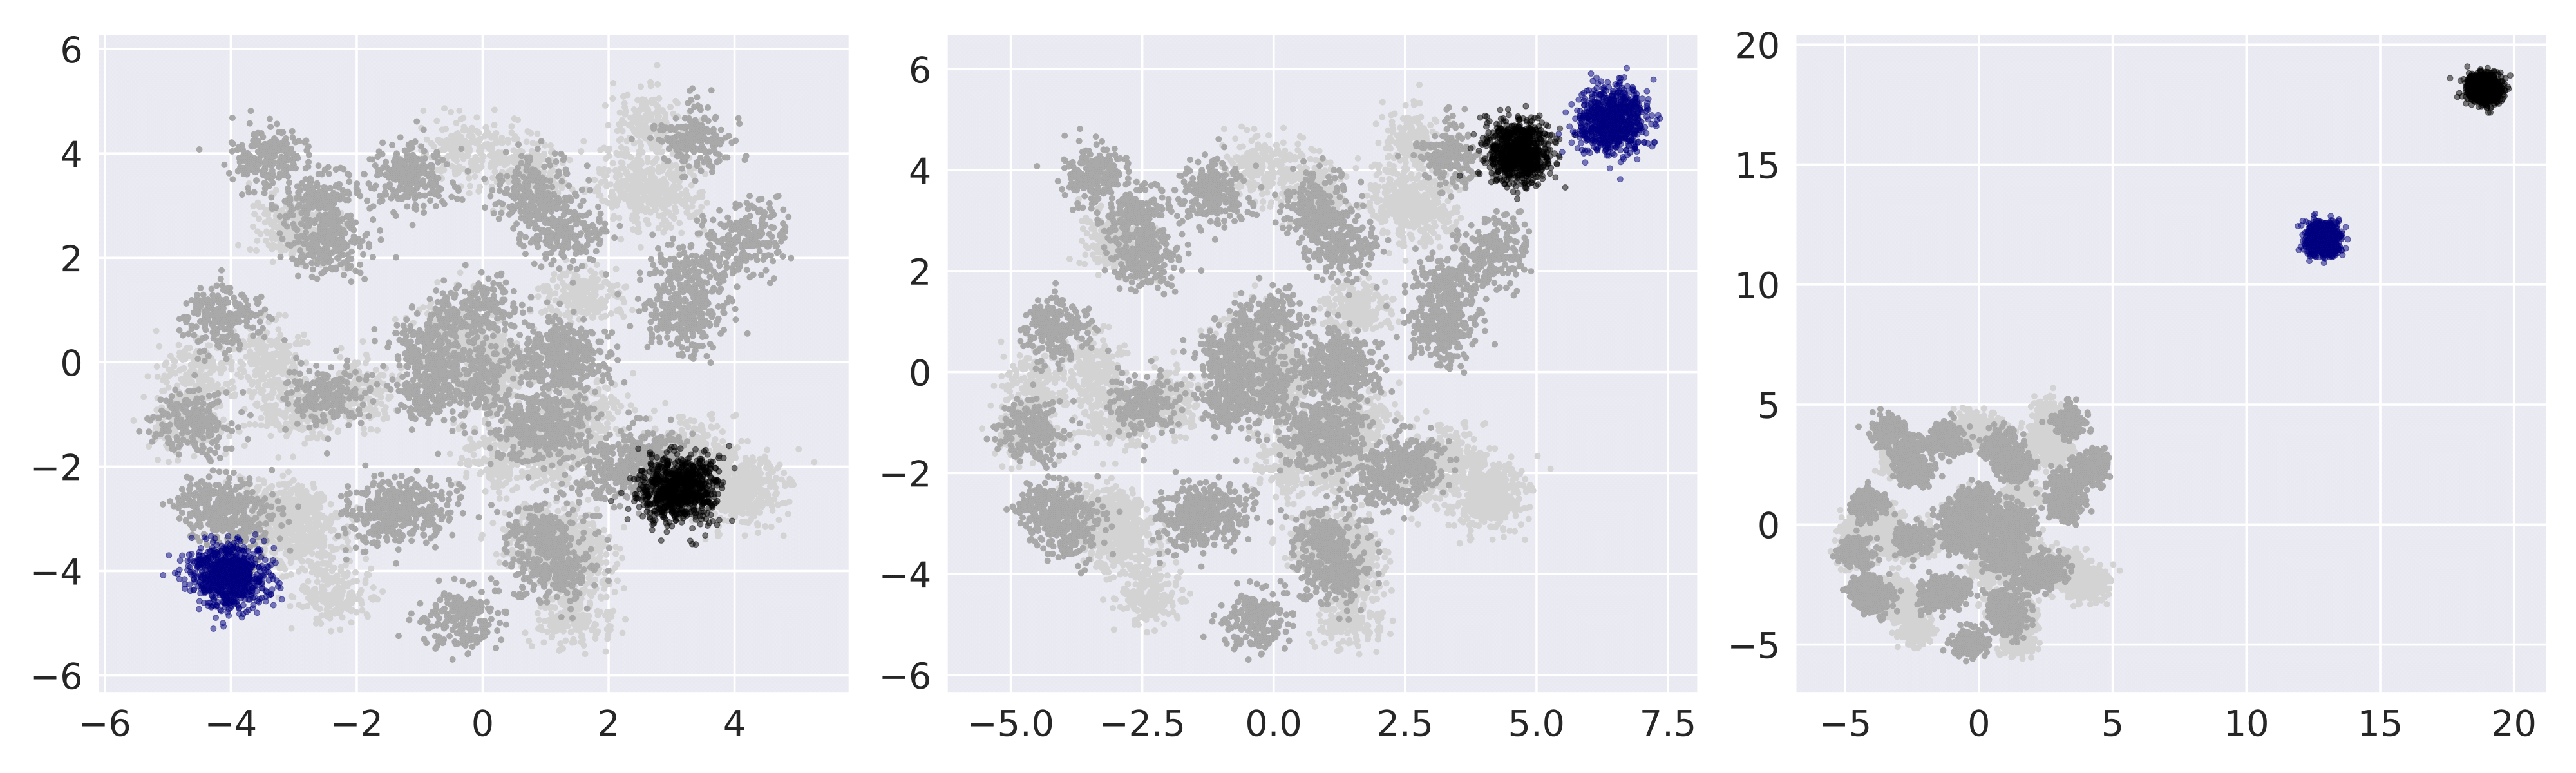
\includegraphics[width=\linewidth]{images/chapter5/mixtures/generalization_schemes.png}
\caption{Thirty mixtures drawn from the meta-distribution $\mathcal{M}$. We plot (in color) 3 unseen distributions whose parameters are drawn from (left) $U(-5, 5)$; (middle) $U(3,7)$; (right) $U(10, 20)$, the first two begin in and close to $\mathcal{M}$ whereas the last mixture is clearly outside of $\mathcal{M}$.}
\label{fig:mnist:gen}
\end{figure}

Next, we investigate clustering ability of the meta-inference model on mixture distributions outside of $p_{\mathcal{M}}$ as we vary the amount of fine-tuning data (previously, we did not allow any fine-tuning -- inference was zero-shot). See Figure~\ref{fig:mnist:gen} for different measures of generalizability. Specifically, we extract the pre-trained meta-inference model and train a new generative network on each of 3 unseen data distributions, evaluating the clustering performance. We only use \{5, 10, 15, 20\}\% of the test distribution for training. As shown in Figure~\ref{fig:extra:mnist}(a), the model is able weakly generalize across all levels of meta-training, outperforming the VAE baseline with the exception of the 100 GMM meta-encoder -- a phenomena consistent with the results shown in Table 1, i.e., overfitting to the meta-training set. However, Figure~\ref{fig:extra:mnist}(b,c) shows that meta-training does not seem to provide significant gains in generalization performance on marginals far from $p_{\mathcal{M}}$, again consistent with other demonstrations.

\begin{figure}
\centering     %%% not \center
\begin{subfigure}[b]{0.32\linewidth}
    \includegraphics[width=\linewidth]{images/chapter5/mixtures/unseen_metadist_clustering.pdf}
    \caption{$\mu \sim U(-5, 5)$}
\end{subfigure}
\begin{subfigure}[b]{0.32\linewidth}
    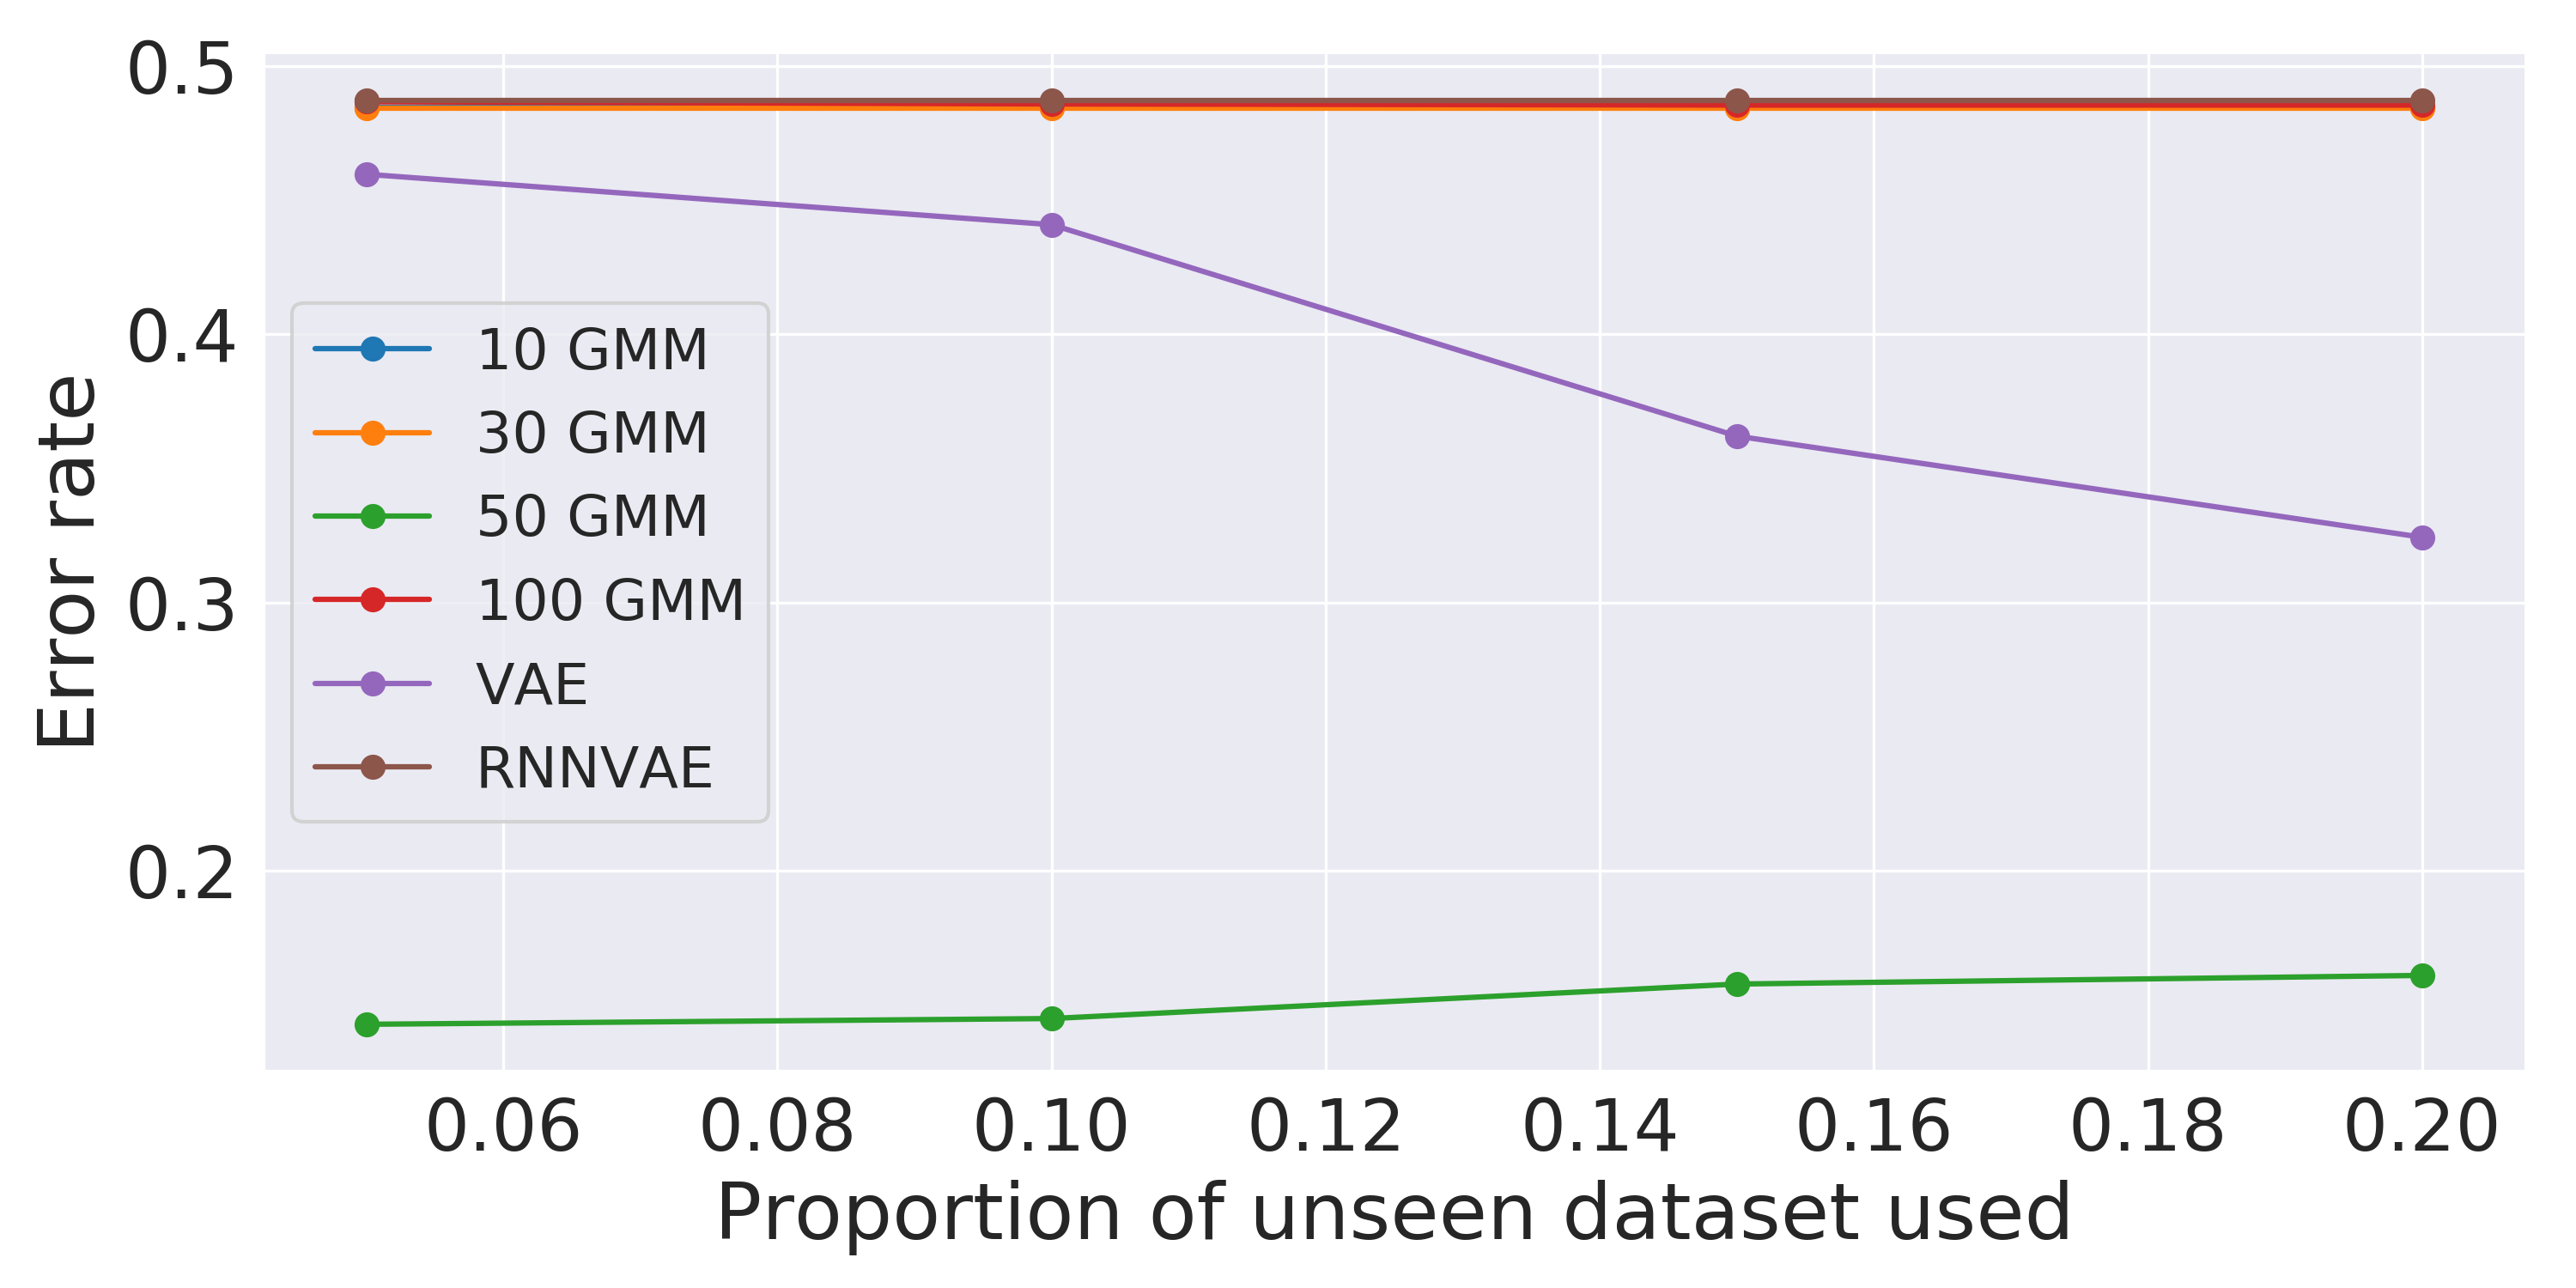
\includegraphics[width=\linewidth]{images/chapter5/mixtures/unseen_3_7_clustering.pdf}
    \caption{$\mu \sim U(3, 7)$}
\end{subfigure}
\begin{subfigure}[b]{0.32\linewidth}
    \includegraphics[width=\linewidth]{images/chapter5/mixtures/unseen_10_20_clustering.pdf}
    \caption{$\mu \sim U(10, 20)$}
\end{subfigure}
\caption{Clustering performance after training on \{5,10,15,20\}\% of the unseen data distribution. In (a), meta-training on 10, 30, and 50 datasets allows for perfect clustering, outperforming the VAE. In (b), only the 50 GMM meta-trained model has successfully learned to cluster. In (c), the meta-clustering algorithm fails to generalize to an extremely out-of-sample distribution.}
\label{fig:extra:mnist}
\end{figure}

\subsubsection{Clustering Handwritten Digits}

Next, we construct a setup analogous to the mixtures of Gaussians experiment with MNIST digits \cite{lecun1998mnist}. Specifically, we hold out two digit classes for out-of-sample evaluation, and generate datasets comprised of pairs of the remaining digits. We select a subset of \{5, 10, 20\} combinations out of a total of 28 (8 choose 2) possibilities to train the MetaVAE. We then ask the model to cluster new digit pairs, either drawn from the eight unseen pairs in $\mathcal{M}$ or the digit pair (3s and 7s) that were held out completely in training. We use continuous 40-dimensional latent variables to better model the complexity of the data.

Like in MoG, we use MetaVAE representations to train a logistic regression model with the true labels (0/1 for each digit class). 
% Intuitively, logistic regression finds the best linear split between two clusters in the latent space; note that for it to perform well, such a linear split must already exist. 
To measure performance, we embed the test set and compare against true labels. Fig.~\ref{fig:mnist}(a,b) shows the clustering results for two levels of difficulty: digit pair (1,6) (visually easy) and (4,9) (visually hard). For the former, an MetaVAE outperforms the VAE trained on the \textit{full} dataset of 1's and 6's. For the more difficult task, adding more combinations improves clustering performance, and the MetaVAE outperforms a VAE trained on half of the target data. Fig.~\ref{fig:mnist}(c) shows MetaVAE performance on the out-of-sample digit pair (3,7). The MetaVAE obtains less than 2\% clustering error \textit{without additional gradient steps}. Further, surprisingly, it outperforms a VAE which has been trained on 100\% of the target dataset of 3's and 7's. 
% We note that the MetaVAE has inferred useful representations that allows for good zero-shot clustering performance on a new, unseen dataset.
\begin{figure}
\centering
\begin{subfigure}[b]{0.32\linewidth}
    \includegraphics[width=\linewidth]{images/chapter5/mnist/weak_gen_clustering_err_vae_baseline_1_6.pdf}
    \caption{Digit Pair (1,6)}
\end{subfigure}
\begin{subfigure}[b]{0.32\linewidth}
    \includegraphics[width=\linewidth]{images/chapter5/mnist/weak_gen_clustering_err_vae_baseline_4_9.pdf}
    \caption{Digit Pair (4,9)}
\end{subfigure}
\begin{subfigure}[b]{0.32\linewidth}
    \includegraphics[width=\linewidth]{images/chapter5/mnist/strong_gen_clustering_err_vae_baseline.pdf}
    \caption{Digit Pair (3,7)}
\end{subfigure}
\caption{Clustering on MNIST digit pairs. We train a MetaVAE amortized over \{5, 10, 20\} pairs of digit classes and evaluate their performance on unseen pairs from and outside of  $p_\mathcal{M}$. (a,b) shows that the MetaVAE achieves higher clustering accuracy compared to a VAE trained on 100\% and 50\% of the target distribution (within $p_\mathcal{M}$). (c) shows that the MetaVAE outperforms a VAE trained on 100\% of the out-of-sample distribution (not in $p_\mathcal{M}$).}
\label{fig:mnist}
\end{figure}

\subsubsection{Classical Mechanics (Continued)}

We include the derivation for the meta-compiled inference objective from the main text. Note that this is very similar to \cite{le2016inference}.

\begin{align*}
    L_\phi &= \mathbf{E}_{p_{\theta_i^*}(x)}[D_{\text{KL}}(p_{\theta_i^*}(z|x)) || g_\phi(z|p_{\theta_i^*}, x))] \\
    &= \int_{x} p_{\theta_i^*}(x) \int_{z} p_{\theta_i^*}(z|x)\log \frac{p_{\theta_i^*}(z|x)}{g_\phi(z|p_{\theta_i^*}, x)} dz dx \\
    &\propto \mathbf{E}_{p_{\theta_i^*}(x, z)}[-\log g_\phi(z|p_{\theta_i^*}, x)]
\end{align*}

\subsubsection{Distribution Statistics Details}
As this experiment setup is slightly involved, we provide a more thorough explanation with details here. 

Recall that a sufficient statistic is defined as a function $\phi(x)$ mapping realizations of a random variable to a vector in $\mathbf{R}^d$. We noted in the main text that for realizations of a ``random vector" (length $k$) whose entries each are a random variable distributed i.i.d. according to some exponential family, the sum $\sum_{i=1}^k \phi(x_i)$ of the sufficient statistics for realizations of each random variable in the vector. Finally, recall that the objective is: having seen many realizations of random vectors from different exponential family distributions, is it possible to learn a sufficient statistic for a new random vector that can be used to estimate the parameters of the (possibly unseen) underlying distribution that each random variable in the vector is distributed by?

If we treat an observation $x$ as a realization of a random vector, then the meta-inference model $g_\phi(p_{\textup{data}}, x)$, as a function of $x$, should act as a sufficient statistic for $p_{\textup{data}}$. A key distinction between the this experiment and the mixture of Gaussians (MoG) experiment is what an observation represents. In MoG, we represent the $i$-th observation $x_i$ as a 2-D vector sampled from a mixture distribution; when doubly amortizing, the meta-inference model $g_\phi$ takes as input $x_i$ and a marginal distribution, which we represent as a data set $\textup{data}_i = \{ x \}_i$. In contrast, in this experiment, the $i$-th observation is interpreted as a \textit{realization of a random vector} $x$. The meta-inference model $g_\phi$ still takes as input the observation and a marginal distribution. 

In this case, the marginal is a distribution over random vectors, which we represent as a set of realizations (samples) of random vectors. We studied four different cases (meta-distributions): \textbf{1) First,} we perform inference for all two dimensional Gaussian distributions with spherical covariance of 0.1 and a mean between -5 and 5. This implies that every random vector will be composed of i.i.d samples from a 2-D Gaussian distribution. The inference objective is estimate the unknown parameters of a new unseen Gaussian distribution after training. \textbf{2) Second,} we consider all two dimensional Log Normal distributions with spherical covariance of 0.1 and a mean between -5 and 5. \textbf{3) Third,} we consider all two dimensional Exponential distributions with scale less than 5. \textbf{4) Fourth,} we consider the union of distributions in the previous three cases (this defines the largest meta-distribution of the four cases). Note that each distribution defined above only has one free (continuous) parameter, which will serve as the statistic that we infer.

In each case, we must construct a meta-training and meta-test set where the former is used to train the MetaVAE and the latter is used to measure generalization of inference. To create the meta-training set, we randomly sampled 30 parameters defining 30 distributions (for example, sample 30 means from a uniform distribution $U(-5, 5)$ to define 30 Gaussian distributions). For each of the 30 distributions, we sample 20 times, building a 20-D random vector $x$. To represent the marginal distribution, we use a set of 10 random vectors, each sampled  i.i.d. For the meta-test set, we consider an interpolation of unseen distributions across a range of parameters. For example, for the first case of only amortizing over Gaussian distributions, we meta-test on Gaussians with means from -10 to 10 by 0.1 increments. By also considering means outside of -5 and 5 (the meta-distribution), we measure how well the MetaVAE can do inference in and outside of the meta-distribution. A similar design is used for cases 2 through 4. 

Next, we describe components of the MetaVAE. We place the full burden of learning onto the meta-inference model by making each generative model $p_{\theta_i}(x|z)$ parameter-free i.e. $g_\phi$ has no choice but to act as the sufficient statistic; Critically, this is possible since $p_{\theta_i}(x|z)$ is given the correct distributional family that $p_{\textup{data}_i}(x)$ belongs to (so it knows how to use $z$ to define a distribution). Knowing the correct distributional family also defines the loss function; for example, if we are given that $p_{\textup{data}_i}(x)$ is Gaussian, then $z$ represents the mean and we can use a Gaussian PDF in the lower bound computation. However, the meta-inference model $g_\phi(p_{\textup{data}_i}, z)$ is tasked with matching marginals with the correct families and must produce a latent variable $z$ to capture the parameters of the true distribution, $p_{\textup{data}_i}(x)$. Since the number (1) and dimensionality (2) of all sufficient statistics are identical, we can choose $z$ to be a two dimensional continuous random variable. Future work can explore more complex designs such as distributions with different numbers of sufficient statistics. For some statistics, we add a Softplus function to ensure that it is greater than 0 (e.g. scale for exponential distributions). In terms of architectures, we chose a multilayer perceptron (MLP) that ingests a set $\{x\}_i$ and outputs a set of hidden vectors that we average over into a single hidden vector. This network is used to reduce an observation (set of sample vectors from a distribution) into a single vector $h_i$ as well as the representation of the marginal distribution into a set of vectors, $\{h\}_i$. Together, $h_i$ and $\{h\}_i$ are ingested by a separate MLP to return variational parameters for the sufficient statistic. 

At test time, no additional training is needed to do inference for unseen distributions. For an unseen distribution, we use the meta-inference model as a  statistic to estimate the unknown parameter of the given distribution. We report the mean squared error against the true parameter of the underlying distribution, which is known when generating the dataset.

In each of the four cases, we compare our results to baseline models. When amortizing over a single family of distributions (e.g. cases 1 through 3), we compare an doubly-amortized inference procedure with a singly amortized one: we train a VAE on a distribution from the family with a randomly chosen statistic: $[-1.2, 1.1]$ mean for Gaussian, $[-0.5, 1.8]$ mean for Log Normal, $[1.4, 2.8]$ scale for Exponential. The goal of this baseline is to see how inference generalizes without amortizing over generative models (poorly as it turns out). For case 4, when considering multiple families from the Exponential families, we compare a MetaVAE amortized over 30 Gaussian, 30 Log Normal, and 30 Exponential distributions (for a total of 90 distributions) to three separate MetaVAEs, amortized over only 30 distributions of its family e.g. 30 Gaussians, 30 Log Normals, and 30 Exponentials respectively. Including these baselines again measures the effect of meta-amortization. Finally, in main text, we also tested how well inference works for other members of Exponential family that were not observed during training. To be specific, we included Weibull distributions with scale 1 and shapes from $[0,5]$, Laplace distributions with location 0 and scales in $[0,5]$, and ``symmetric" Beta distributions with two equal shape parameters from $[0,5]$.

\begin{figure}
\centering     %%% not \center
\begin{subfigure}[b]{0.49\linewidth}
    \includegraphics[width=\linewidth]{images/chapter5/toy_gaussian/gaussian_only_test_set_mu.png}
    \caption{}
\end{subfigure}
\begin{subfigure}[b]{0.49\linewidth}
    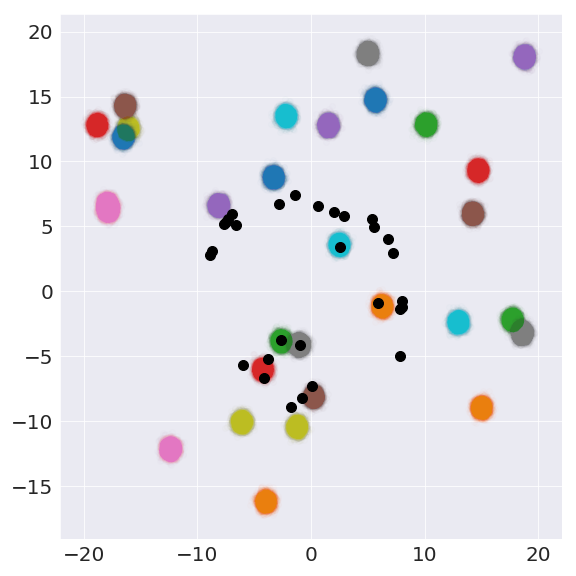
\includegraphics[width=\linewidth]{images/chapter5/toy_gaussian/gaussian_only_out_of_sample_set_mu.png}
    \caption{}
\end{subfigure}
\begin{subfigure}[b]{0.49\linewidth}
    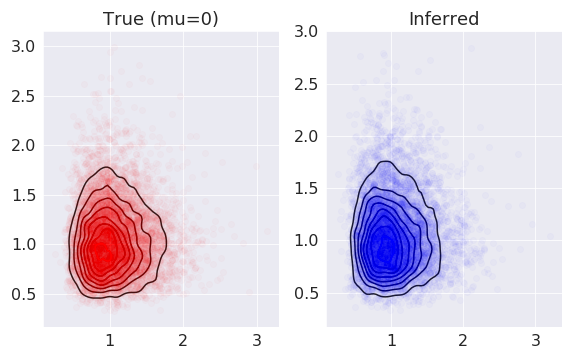
\includegraphics[width=\linewidth]{images/chapter5/toy_gaussian/lognormal_exapmle_good.png}
    \caption{Log Normal}
\end{subfigure}
\begin{subfigure}[b]{0.49\linewidth}
    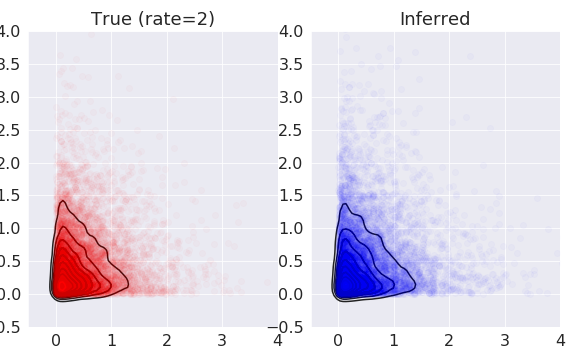
\includegraphics[width=\linewidth]{images/chapter5/toy_gaussian/exponential_exapmle_good.png}
    \caption{Exponential}
\end{subfigure}
\caption{Colored circles represent 30 different $p_{\textup{data}_i} \sim p_{\mathcal{M}}$; black dots represent the inferred Gaussian means from the meta-inference model. (a) Test Gaussian distributions within $\mathcal{M}$; (b) Test distributions outside of $\mathcal{M}$. (c,d) Samples from the an unseen Log Normal or Exponential distribution $p_{\textup{data}_i} \in p_{\mathcal{M}}$ (red) and the true corresponding distribution defined by the inferred statistic (blue).}
\label{fig:gaussian_plot}
\end{figure}

\subsubsection{Architectures}

In the main text, recall that $g_\phi(p_{\textup{data}_i}, x)$ is a supervised doubly amortized regressor that takes as input a marginal distribution $p_{\textup{data}_i}$ and an observation $x$ to return a posterior distribution. In practice, we need additional machinery to parameterize $g_\phi(p_{\textup{data}_i}, x)$ with neural networks. For some dataset $D_i$ and $x \in \mathcal{X}$, we set $\hat{g}_\phi(D_i, x) = r_{\psi}(\textsc{concat}(x, h_{\gamma}(D))$ where $\phi = \{ \psi, \gamma \}$, $h(\cdot)$ is \textit{summary} neural network that ingests the elements in $D$, and $r(\cdot)$ is an \textit{aggregation} neural network that ingests the input and the summary.

\paragraph{Mixture of Gaussians Experiment} The inference network for both the VAE and the MetaVAE is composed of 3 linear layers (hidden dimensions of 10) with ReLU nonlinearity in between each. The decoder networks share the same architecture as well. The summary network for the MetaVAE is also a MLP with three layers (hidden dimensions of 10) and Leaky ReLU nonlinearity.

\paragraph{Classical Mechanics Experiment} The inference model is identical to the MoG experiment except the latent variable is continuous (although still one-dimensional). No decoders are used as the simulators act as fixed generative models. The summary network is also as in MoG. 

%\krsity{@mike TODO}
% \paragraph{Classical Mechanics Experiment} The inference network for both the VAE and the MetaVAE is composed of 3 linear layers (hidden dimensions of 10) with ReLU nonlinearity in between each. The decoder networks share the same architecture as well. The summary network for the MetaVAE is also a MLP with three layers (hidden dimensions of 10) and Leaky ReLU nonlinearity.

\paragraph{Exponential Family Experiment} The inference network is composed 3 linear layers  (hidden dimensions of 400) with ReLU nonlinearity in between each. The summary network is also a MLP with three layers (hidden dimensions of 400) and Leaky ReLU. Results are not sensitive to choices of dimensionality and nonlinearities.

\paragraph{MNIST and NORB Experiments} As many of the components as possible are shared between MetaVAE, NS, ad VHE. The latter two require additional sub-networks to ingest and decode a second (global) latent variables; thus, NS and VHE have more trainable parameters than MetaVAE. 

For MNIST, we use simpler architectures, flattening each image into a 784 dimensional vector. Specifically, we start with 3 linear layers with 400 hidden dimensions and ReLU nonlinearity for the encoder; 3 linear layers with 400 hidden dimensions and ReLU nonlinearity for each decoder; and 3 linear layers with 400 hidden dimensions and ReLU nonlinearity for the summary network. We used 40 latent dimensions (denoted $\mathbf{z}$). For NS and VHE, we used an additional global latent (denoted $\mathbf{c}$) of 300 dimensions and 3 linear layers with 400 hidden dimensions and ReLU nonlinearity to decode latent $\mathbf{z}$ from latent $\mathbf{c}$. 

Since NORB is more difficult (being realistic instead of synthetic images), we trade linear layers for convolutional architectures. Specifically, for the decoder, the MetaVAE uses: a linear layer first to increase the input dimensionality to $256*4*4$, which will be reshaped into an image; followed by six convolutional layers with three transposed convolutional layers every two convolutions with batch normalization after every layer (slowly decreasing the filter size from 256 to 128 to 64 to 1 or 3). For inference, the MetaVAE uses three sub-components: first, we have a large convolutional network with 9 convolutional layers with batch normalization in between layer that ingests the input image and outputs a object of size 256 by 4 by 4. Every input image and every sample from the distribution is processed using this convolutional network. Then the summary network consists of 3 linear layers with 400 hidden dimensions and ReLU nonlinearity that injests the output of the convolutional network into a summary statistic over samples. The resulting summary is concatenated with the output of the convolutional network for the input image and fed into two linear layers (400 hidden dimensions) with residual connections that spit out parameters of a Gaussian distribution over latent $z$. Again, VHE and NS have a second global latent variable of 300 dimensions that requires a separate decoder network, which we now define with two linear layers with residual connections (400 hidden dimensions).

\subsubsection{Hyperparameters}
\paragraph{Mixture of Gaussians Experiment} For the MetaVAE, we used a batch size of 20, a learning rate of 2e-4, and trained for 500 epochs using the Adam optimizer. For the VAE, we used a batch size of 100, a learning rate of 1e-3, and trained for 200 epochs using the Adam optimizer. The dataset was generated by sampling the appropriate MoG, where we sampled means uniformly from the ranges such as $U(-5, 5)$. We doubly-amortize over \{10, 30, 50\} such datasets at one time. We trained the model by exact enumeration of the ELBO/MetaELBO to avoid high-variance gradient estimates induced by using a 1-D discrete latent variable $\mathbf{z}$.

\paragraph{Classical Mechanics Experiment} We use a batch size of 64, a learning rate of 2e-4, and trained for 10 epochs using Adam (for both VAE and MetaVAE). The dataset was created by running each simulator in the meta-train set 1000 times (similar for testing). For the VAE baseline we chose the ``center" simulator (a length of 10 in range 1 to 19 and an angle of 45 in range 5 to 85) which should give the best hope of generalization without doubly-amortizing. 

% \kristy{@mike TODO}
% \paragraph{Classical Mechanics Experiment} We used a batch size of 20, a learning rate of 1e-3, and trained for 200 epochs using the Adam optimizer. The dataset was generated by sampling 1000 times i.i.d. from a parameterized distribution in the exponential family. We doubly-amortize over 10 to 30 such datasets at one time. The latent dimension was chosen to match the number of sufficient statistics and 20 i.i.d. samples where given to the summary network.

\paragraph{Exponential Family Experiment} We used a batch size of 20, a learning rate of 2e-4, and trained for 100 epochs using the Adam optimizer. The dataset was generated by sampling 1000 times i.i.d. from a parameterized distribution in the exponential family. We doubly-amortize over 10 to 30 such datasets at one time. The latent dimension was chosen to match the number of sufficient statistics and 20 i.i.d. samples where given to the summary network.

\paragraph{MNIST and NORB Experiments} We used a batch size of 100, a learning rate of 2e-4, and trained for 100 epochs using the Adam optimizer. MNIST images were kept at 28 by 28 pixels whereas NORB images were resized and center cropped to 32 by 32 pixels. All generative models used a latent dimension of 40 and 10 i.i.d. samples from the dataset to represent the distribution as input to $\hat{g}_{\phi}$. 


\section{Chapter~\ref{chapter:foundation}}

We provide supplemental descriptions, experiments, and analysis below.

\subsection{Additional Figures}

Figure~\ref{fig:data} shows an example of annotating a probabilistic program and randomly masking assigned observations from three different executions.

\begin{figure}[h!]
  \centering
  \begin{subfigure}[b]{0.40\textwidth}
    \includegraphics[width=\textwidth]{images/chapter6/mask_process.png}
    \caption{}
  \end{subfigure}
  \hfill
  \begin{subfigure}[b]{0.49\textwidth}
    \centering
    \includegraphics[width=\textwidth]{images/chapter6/mask_examples.png}
    \caption{}
  \end{subfigure}
  \caption{On the left, a standard probabilistic program is reformatted such that \texttt{observe} statements are replaced with annotations. On the right are 3  executions with randomly masked variables.}
  \label{fig:data}
\end{figure}

\subsection{Toy Experiments}
\label{sec:app:mli}

We begin by providing a high level description of the six probabilistic programs used in the main text. Following this, we will provide the pseudocode.

\paragraph{Latent} Two Gaussian random variables, $\mathcal{N}(\mu_1, \sigma^2_1)$ and $\mathcal{N}(\mu_2, \sigma^2_2)$ where $\mu_2$ is a random affine function of a sample $z_1 \sim \mathcal{N}(\mu_1, \sigma^2_1)$. We choose $\sigma_1 \sim \mathcal{U}(0, 20)$, $\sigma_2 \sim \mathcal{U}(0.5, 10)$.

\paragraph{Clustering} Two samples $z_1,z_2 \sim \mathcal{N}(0, 100)$ are divided into two groups $g_1 \sim \mathcal{N}(\mu_1, \sigma^2_1)$ or $g_2 \sim \mathcal{N}(\mu_2, \sigma^2_2)$ using an \texttt{if} statement. We choose $\mu_1, \mu_2 \sim \mathcal{N}(-15, 15)$ and $\sigma_1, \sigma_2 \sim \mathcal{U}(0.5, 50)$.

\paragraph{Hierarchical} Three random variables $g \sim \mathcal{N}(\mu_g, \sigma^2_g)$, $t \sim \mathcal{N}(g, \sigma^2), z \sim \mathcal{N}(t, \sigma^2)$ each with a mean chosen as a sample from the parent. We choose $\mu_g \sim \mathcal{U}(-5, 5), \sigma_g \sim \mathcal{U}(0, 50), \sigma \sim \mathcal{U}(0, 10)$.

\paragraph{Multi-level} Similar to \textit{Hierarchical} but child random variables are modelled as a regression of parent samples where slope and intercept are randomly chosen.

\paragraph{Milky way} A probabilistic model for the velocity of two sallite galaxies $v_1 \sim \mathcal{N}(m \times 2, 5), v_2 \sim \mathcal{N}(m + 5, 2)$. The log mass $m$ of the Milky Way is sampled from $N(5, 10)$.

\paragraph{Rosenbrock} Computes a noisy Rosenbrock function on samples from two Gaussian variables. The Rosenbrock function is treated as a library import and its code is not provided to the model.\newline

We more thoroughly describe the toy probabilistic programs used in Section~\ref{sec:toyexpt}. An equivalent description can be found on pages 17-20 in \url{https://arxiv.org/pdf/2103.00737.pdf}. Consider the following pseudocode: 

\paragraph{Latent} $\mu_1 \sim \mathcal{U}(-5, 5); \sigma_1 \sim \mathcal{U}(0, 20); z_1 \sim \mathcal{N}(\mu_1, \sigma^2_1); c_1 \sim \mathcal{U}(-3 3); z_2 = z_1 \times c_1; c_2 \sim \mathcal{U}(-10, 10); z_3 = z_2 + c_2; \sigma_2 \sim \mathcal{U}(0.5, 10); z_4 \sim \mathcal{N}(z_3, \sigma^2_2)$.

\paragraph{Clustering} $\mu_1 \sim \mathcal{U}(-15, 15); \sigma_1 \sim \mathcal{U}(0.5, 50); g_1 \sim \mathcal{N}(\mu_1, \sigma^2_1); \mu_2 \sim \mathcal{U}(-15, 15); \sigma_2 \sim \mathcal{U}(0.5, 50); g_2 \sim \mathcal{N}(\mu_2, \sigma^2_2); t_1 \sim \mathcal{N}(0, 100); m_1 = \texttt{ if } (t_1 > 0) g_1 \texttt{ else } g_2; \sigma_3 \sim \mathcal{U}(0.5, 10); z_1 \sim \mathcal{N}(m_1, \sigma^2_3); t_2 \sim \mathcal{N}(0, 100); m_2 = \texttt{ if } (t_2 > 0) g_1 \texttt{ else } g_2; z_2 \sim \mathcal{N}(m_2, \sigma^2_3)$.

\paragraph{Hierarchical} $\mu_1 \sim \mathcal{U}(-5, 5); \sigma_1 \sim \mathcal{U}(0, 50); g \sim \mathcal{N}(\mu_1, \sigma^2_1); \sigma_2 \sim \mathcal{U}(0, 10); t_1 \sim \mathcal{N}(g, \sigma^2_2); \sigma_3 \sim \mathcal{U}(0, 10); t_2 \sim \mathcal{N}(g, \sigma^2_3); \sigma_4 \sim \mathcal{U}(0.5, 10); z_1 \sim \mathcal{N}(t_1, \sigma^2_4); \sigma_5 \sim \mathcal{U}(0.5, 10); z_2 \sim \mathcal{N}(t_2, \sigma^2_5)$.

\paragraph{Multi-Level} $\mu_1 \sim \mathcal{U}(-10, 10); \sigma_1 \sim \mathcal{U}(0, 100); a_0 \sim \mathcal{N}(\mu_1, \sigma^2_1); \sigma_2 \sim \mathcal{U}(0, 10); a_1 \sim \mathcal{N}(a_0, \sigma^2_2); \sigma_3 \sim \mathcal{U}(0, 10); a_2 \sim \mathcal{N}(a_0, \sigma^2_3); \mu_2 \sim \mathcal{U}(-5, 5); \sigma_4 \sim \mathcal{U}(0, 10); b \sim \mathcal{N}(\mu_2, \sigma^2_4); c_1 \sim \mathcal{U}(-5, 5); t_1 = b \times c_1; t_2 = a_1 + t_1; \sigma_5 \sim \mathcal{U}(0.5, 10); z_1 \sim \mathcal{N}(t_2, \sigma^2_5); c_2 \sim \mathcal{U}(-5, 5); t_3 = b \times c_2; t_4 = a_2 + t_3; \sigma_6 \sim \mathcal{U}(0.5, 10); z_2 \sim \mathcal{N}(t_4, \sigma^2_6)$.

\paragraph{Milky Way} $\mu_1 \sim \mathcal{U}(-10, 10); \sigma_1 \sim \mathcal{U}(0, 30); m_0 \sim \mathcal{N}(\mu_1, \sigma^2_1); c_1 \sim \mathcal{U}(-2, 2); m_1 = m_0 \times c_1; \sigma_2 \sim \mathcal{U}(0, 10); g_1 \sim \mathcal{N}(m_1, \sigma^2_2); c_2 \sim \mathcal{U}(-5, 5); m_2 = m_0 + c_2; \sigma_3 \sim \mathcal{U}(0, 10); g_2 \sim \mathcal{N}(m_2, \sigma^2_3); \sigma_4 \sim \mathcal{U}(0.5, 10); z_1 \sim \mathcal{N}(g_1, \sigma^2_4); \sigma_5 \sim \mathcal{U}(0.5, 10); z_1 \sim \mathcal{N}(g_2, \sigma^2_5)$.

\paragraph{Rosenbrock} $\mu_1 \sim \mathcal{U}(-8, 8); \sigma_1 \sim \mathcal{U}(0, 5); z_1 \sim \mathcal{N}(\mu_1, \sigma^2_1); \mu_2 \sim \mathcal{U}(-8, 8); \sigma_2 \sim \mathcal{U}(0, 5); z_2 \sim \mathcal{N}(\mu_2, \sigma^2_2); r = \texttt{rosenbrock}(z_1, z_2); \sigma_3 \sim \mathcal{U}(0.5, 10); z_3 \sim \mathcal{N}(r, \sigma^2_3)$.

\paragraph{Hyperparameters and Training Details} A dataset of $10\,000$ examples are generated by re-executing the probabilistic program. A separate dataset of $1\,000$ examples are generated and held-out in training. For the transformer, we use a RoBERTa
\cite{liu2019roberta} architecture, a maximum length of 200, linear learning rate scheduling with $5\,000$ warmup steps, and finetune only the top 6 transformer layers. In the loss, we set $\alpha = 0.1$, the weight on the loss from the inference head. In optimization, we use Adam \cite{kingma2014adam} with a batch size of 16, a learning rate of 4e-3, clip gradients norms at max 1, for 300 epochs. We take the checkpoint with the best loss on a dev set for test evaluation.

\paragraph{Additional Analysis}

We note that for half of the toy programs (especially, hierarchical or multi-level), the variance of log IW is noticeably higher than for the other programs. This pattern persists for the ablation. To study this more, we visualize the histogram of log IWs for the standard MLI and ablation on the `hierarchical' program in Figure~\ref{fig:vliw}. We observe that the majority of the test runs result in log IWs near zero, meaning high quality inference. However, there are a number of examples that the log IW is significantly higher for. The trained MLI model does not generalize as well to these points. Without the MLM loss, we observe these ``difficult'' cases to be more frequent and severe. In the right subfigure, we ommited points with log IW $>1\,000$ for visibility.

\begin{figure}[h!]
  \centering
  \begin{subfigure}[b]{0.49\textwidth}
    \centering
    \includegraphics[width=0.8\textwidth]{images/chapter6/vliw_hist.pdf}
    \caption{With MLM}
  \end{subfigure}
  \hfill
  \begin{subfigure}[b]{0.49\textwidth}
    \centering
    \includegraphics[width=0.8\textwidth]{images/chapter6/vliw_hist_no_mlm.pdf}
    \caption{Without MLM}
  \end{subfigure}
  \hfill
\caption{With and without the MLM loss, we see the majority of the log IWs are near zero, suggesting high quality inference. However, there are a number of data points for which the log IW is higher. We observe this to be more frequent and more severe without MLM.}
\label{fig:vliw}
\end{figure}

\subsection{Visualizing Attention}
\label{sec:app:viz}

We provide more details on the programs and additional results.

\paragraph{Independent Gaussians} $\mu_1 \sim \mathcal{U}(-5, 0); \sigma_1 \sim \mathcal{U}(0, 5); z_1 \sim \mathcal{N}(\mu_1, \sigma^2_1); \mu_2 \sim \mathcal{U}(0, 5); \sigma_2 \sim \mathcal{U}(0, 5); y_1\sim \mathcal{N}(\mu_2, \sigma^2_2); z_2 = z_1 \times 2; y_2 = y_1 \times 2$. We expect $z_2 \perp y_2$ and $z_1 \perp y_1$.

\paragraph{Conditional Independence} $p \sim \mathcal{U}(0, 1); z \sim \textup{Bern}(p); a = \texttt{ if }(z = 1) 1 \texttt{ else } 10; b = \texttt{ if }(z = 1) 3 \texttt{ else } -3; x \sim \mathcal{N}(a, 1); y \sim \mathcal{N}(b, 1)$. We expect $x \perp y | z, a \perp b | z$.

\paragraph{Common Effect} $p_x \sim \mathcal{U}(0, 1); p_y \sim \mathcal{U}(0, 1); x \sim \textup{Bern}(p_x); y \sim \textup{Bern}(p_y); z = \texttt{ if }(x \texttt{ or } y) 1 \texttt{ else } 0$. We expect that knowing both $y$ and $z$ should determine $x$.
% We expect $x \perp y|z$ but we expect that observing $y$ and $z$ explains away $x$ (i.e. creates a dependency between $x$ and $y$).

\paragraph{Tabular Results} We include a table reporting log probability and variance of log IW for the three programs above. As these are ``simpler'' programs than even those in the MLI toy experiments, we observe more favorable results.

\begin{table}[h!]
\centering
\begin{tabular}{lcc}
\toprule
Program & \multicolumn{2}{c}{Test Set Evaluation} \\
& $\log p(z|x)$ & $\text{var}\left\{\log \frac{p(x,z)}{q(z|x)}\right\}$ \\
\midrule
Independent Gaussians & $0.856$ & $0.779$ \\
Conditional Independence & $0.616$ & $0.674$ \\
Common Effect & $1.215$ & $0.889$ \\
\bottomrule
\end{tabular}
\caption{Analogous results to Table~\ref{tab:toy} for the toy problems for visualizing attention.}
\label{tab:toy:viz}
\end{table}

\paragraph{Hyperparameters and Training Details} With the exception of a maximum sequence length of 100, we use the same hyperparameters as in Appendix~\ref{sec:app:mli}.

\subsection{Importance Weights}
We review how to derive log importance weights. Assume an observed variable $x$ and a latent variable $z$. Fix a realization $x \sim p(x)$ from some data distribution $p$. Then $\log p(x) = \log \sum_z p(x,z) = \log \left( \sum_z q(z|x) \left(\frac{p(x,z)}{q(z|x)}\right)\right) = \log \left( \mathbf{E}_{q(z|x)}\left[\frac{p(x,z)}{q(z|x)}\right] \right) \geq \mathbf{E}_{q(z|x)}\left[ \log \frac{p(x,z)}{q(z|x)} \right] = \textup{IW}$. The rightmost expression is called a log importance weight. We compute the variance of log importance weights by sampling several $z_1, \ldots, z_n \sim q(z|x)$ and computing $\textup{Variance}\{ \log\frac{p(x,z)}{q(z|x)}, z \in \{z_1, \ldots z_n\} \}$. The better the importance distribution $q$, the smaller the variance. Observe that if $q(z|x) = p(z|x)$, meaning the approximate posterior is indeed the true posterior, then $\textup{IW} = \mathbf{E}_{p(z|x)}\left[ \log \frac{p(x,z)}{p(z|x)} \right] = \mathbf{E}_{p(z|x)}\left[ \log p(x) \right] = \log p(x)$, a constant. The variance of a constant independent of $z$ is 0.

\subsection{Additional Results for MLI}

In addition to the results in Table~\ref{tab:toy}, we include an additional ablation in Table~\ref{tab:toy} where the weights of the transformer backbone are initialized using CodeBERT \cite{feng2020codebert} rather than RoBERTa (the default).

\begin{table}[h!]
\centering
\begin{tabular}{lcccc}
\toprule
Program & \multicolumn{2}{c}{Ablation: CodeBERT} \\
& $\log p(z|x)$ & $\text{var}\left\{\log \frac{p(x,z)}{q(z|x)}\right\}$ \\
\midrule
Latent & $-1.428${\tiny$\pm 0.1$} & $5.01${\tiny$\pm 2.7$} \\
Clustering & $-3.263${\tiny$\pm 0.2$} & $4.962${\tiny$\pm 4.3$} \\
Hierarchical & $-3.691${\tiny$\pm 0.0$} & $30.59${\tiny$\pm 17$} \\
Multi-level & $-3.054${\tiny$\pm 0.1$} & $69.47${\tiny$\pm 16$} \\
Milky way & $-2.571${\tiny$\pm 0.0$} & $38.07${\tiny$\pm 34$} \\
Rosenbrock & $-2.041${\tiny$\pm 0.2$} & $11.36${\tiny$\pm 4.8$} \\
\bottomrule
\end{tabular}
\caption{Ablation of MLI on the six toy probabilistic programs. We initialize the transformer backbone with CodeBERT rather than RoBERTa.}
\label{tab:toy}
\end{table}
We observe lower variance than with RoBERTa, suggesting that CodeBERT is a viable (perhaps preferrable) alternative. 
% For all STAN experiments, we use CodeBERT.

\subsection{Scientific Notation}

We attempted to structure the inference head $h$ to output scientific notation: output two numbers $a \times 10^b$. The potential upside of this design is more resilience to outliers as it requires a smaller change to represent a difference in magnitude of order. However, we found both instability in training as well as worse average performance. This was due to a one-off error in $b$. Note that being off by one unit in $b$ represents an entire magnitude of order. Future work can explore more stable representations of real numbers. For this paper, we opted for the direct representation in lieu of scientific notation.

\subsection{Toy Experiment with Plating}
\label{sec:app:irt}

To measure the impact of plating with finetuning, we study a toy experiment with item response theory (IRT) \cite{edgeworth1888statistics,hambleton1991fundamentals,rasch1993probabilistic,wu2020variational,wu2021modeling}, which estimates student ability (a latent variable) using student responses (the observations) to an exam via a generative model. The Rasch model \cite{rasch1993probabilistic} says:
\begin{equation}
  p(\texttt{response}_{ij} = 1 | \texttt{ability}_i, \texttt{difficulty}_j) = \texttt{sigmoid}(\texttt{ability}_i - \texttt{difficulty}_j)
  \label{eq:irt}
\end{equation}
where $\texttt{ability}_i$ is the ability of the $i$-th student; $\texttt{difficulty}_j$ is the difficulty level of the $j$-th question; and $\texttt{response}_{ij}$ is the binary correctness of the $i$-th student's response to the $j$-th question.
% These three random variables are all one-dimensional.

We highlight that both difficulty and ability are unknown, which makes inference hard as many choices of ability and difficulty result in the same difference (and hence probability). In practice, every student answers all the same questions, and each student answers multiple questions. With sufficiently many questions, it is possible to triangulate ability accurately.

\begin{figure}[h!]
  \begin{center}
    \includegraphics[width=0.6\linewidth]{images/chapter6/plate_toy.pdf}
  \end{center}
  \caption{Comparison of finetuning to zero-shot on plated IRT.}
  \label{fig:platetoy}
\end{figure}

To set up the toy experiment, we write a probabilistic program where each student answers 30 questions, where $\texttt{ability}_i \sim \mathcal{N}(0, 1)$ and $\texttt{difficulty}_j \sim \mathcal{N}(0, 1)$ are both drawn from standard Gaussians \cite{rasch1993probabilistic}. Next, we generate a dataset of 10k programs by ancestral sampling, and optimize Equation~\ref{eq:mli} (masking random subsets of variables). We do this three times with different minibatch sizes of $k=1$, $2$, and $5$ as thirty responses is too long to fit into 512 tokens (for transformer inputs). Separately, we generate 100 test programs not used in training, masking only the ability variable in each.

We study three different ways to do plated inference for ability: the goal is that during test time, we would like to use all student responses (to the 30 questions) rather than just a minibatch of $k$ questions. We compare finetuning with Equation~\ref{eq:minibatch} to ``zero-shot'', a baseline that infers ability using only $k$ observations. Additionally, we include a stronger zero-shot baseline (called ``product''): for a test program, we build several minibatches, all of size $k$ but composed of different randomly sampled questions. For each minibatch, perform inference for ability, resulting in a posterior Gaussian. Finally, given several Gaussians, apply a product of experts \cite{hinton2002training,wu2018multimodal} to arrive at a final posterior. Figure~\ref{fig:platetoy} plots $\log p(\texttt{ability}_i | \textup{... rest of program ...})$ averaged over test programs for the three approaches. We find that while product improves upon zero-shot performance (by incorporating more information), finetuning achieves higher quality inference still (at the cost of more computation).
% Refer to the Appendix for more details.

\paragraph{Review of Product of Experts} Suppose we are given $k$ Gausian distirbutions. Then, a product of these Gaussian ``experts'' is itself Gaussian \cite{cao2014generalized} with mean $\mu = (\sum_{i} \mu_{i}\text{T}_{i})(\sum_{i}\text{T}_{i})^{-1}$ and covariance $\Sigma = (\sum_{i} \text{T}_{i})^{-1}$, where $\mu_{i}$, $\Sigma_{i}$ are the parameters of the $i$-th Gaussian expert, and $\text{T}_{i} = \Sigma_{i}^{-1}$ is the inverse of the covariance (i.e., the precision).

\begin{table}[h!]
\centering
\begin{tabular}{lcc}
\toprule
Approach & $k$ & $\log p(z|x)$ \\
\midrule
zero shot & 1 & $0.5174$ {\tiny$\pm 0.0122$} \\
zero shot & 2 & $0.6930$ {\tiny$\pm 0.0226$} \\
zero shot & 5 & $1.2824$ {\tiny$\pm 0.0077$} \\
\midrule
product & 1 & $0.7231$ {\tiny$\pm 0.0008$} \\
product & 2 & $0.7707$ {\tiny$\pm 0.1154$} \\
product & 5 & $1.3201$ {\tiny$\pm 0.0858$} \\
\midrule
fientune & 1 & $0.8743$ {\tiny$\pm 0.0069$} \\
fientune & 2 & $1.0836$ {\tiny$\pm 0.0866$} \\
fientune & 5 & $1.7331$ {\tiny$\pm 0.0728$} \\
\bottomrule
\end{tabular}
\caption{Analogous results to Figure~\ref{fig:platetoy} for inferring ability from plated IRT models.}
\label{tab:toy:irt}
\end{table}

\paragraph{Tabular Results} We include a table reporting log probability for the three approaches to inferring ability. This shows the same results as in Figure~\ref{fig:platetoy}.

\paragraph{Hyperparameters and Training Details} We separate the choices for pretraining (MLI) and finetuning. In pretraining, we use a maximum length of 512 and a maximum gradient norm of 5. All other parameters are identical to Appendix~\ref{sec:app:mli}. For the product of experts, we resample minibatches 10 times. In downstream finetuning, we take gradient steps on the top 6 layers of the transformer, initializezd with pretraining weights. We perform a separate optimization for all 100 test programs with batch size of 4, learning rate 4e-3, for 1000 iterations and no gradient clipping. We maintained the linear learning rate scheduler with $5\,000$ warmup steps. These hyperparameters were taken from the default RoBERTa config in Huggingface.

\subsection{Stan Experiments}

We provide a few more details for the Stan experiments. PosteriorDB can be found at \url{https://github.com/stan-dev/posteriordb}. We use the python library \texttt{posteriordb-python}. We filter all posteriors by which ones have ground-truth posterior samples. We remove the following programs: \texttt{arma-arma11}, \texttt{bball\_drive\_event\_0-hmm\_drive\_0}, \texttt{bball\_drive\_event\_1-hmm\_drive\_1}, \texttt{garch-garch11}, \texttt{hmm\_example-hmm\_example}, \texttt{hudson\_lynx\_hare-lotka\_volterra}, \texttt{mcycle\_gp-accel\_gp}, and \newline \texttt{one\_comp\_mm\_elim\_abs-one\_comp\_mm\_elim\_abs}. We randomly chose 3 programs for the test set: \texttt{kidiq-kidscore\_interaction}, \texttt{earnings-logearn\_height}, and \texttt{nes1976-nes}. In pretraining, we generate 10\,000 executions (with randomly masked variables) for each program for a total of 380\,000 training programs. We randomly choose minibatches of size 5 for programs with more observations than can fit within a 512 token sequence. Different executions would result in different minibatches. We initialize the RoBERTa network from HuggingFace pretrained weights, finetuning the top 6 transformer layers using MLI. We set the weight $\alpha = 0.001$. We use batch size 4, learning rate 4e-3, 5\,000 warmup steps, gradient clipping of 1 for 50 epochs. In finetuning, we initialize weights from the foundation posterior and separately optimize for each of the three test programs. All optimization choices stay the same, but we optimize the ELBO objective weighted by the ratio between full observation size and minibatch size. We save checkpoints at 10, 100, and 1000 iterations and record wall clock time at each point.

For Stan NUTS, we use 10 chains, thin set to 10, adaptive delta set to 0.8, and vary the number of sampling and warmup iterations as tuples (100, 50), (200, 100), (500, 200), (1000, 500), (2000, 1000), (5000, 2000), (10k, 5k), (20k, 10k), (50k, 10k). For Stan ADVI, we choose a mean field algorithm, 100 ELBO samples, 1 gradient sample, and vary the number of iterations to be amongst 100, 1k, 5k, 10k, 50k, 100k, 500k, 1M.

\subsection{Resources}

We used a single Titan X GPU for optimizing all deep learning models, with 4-16 CPU background workers for loading data. NUTS and ADVI experiments were run in the same context but without GPU support. We used the PosteriorDB code base \url{https://github.com/stan-dev/posteriordb} for Stan experiments, which has no prohibitive license specified. We used CmdStan-Py for fitting Stan models \url{https://github.com/stan-dev/cmdstanpy} which is licensed under new BSD.

\section{Chapter~\ref{chapter:vibo}}
\label{sec:app:vibo}

\subsection{VIBO Ablation Studies} 
% \bwd{this feels out of place to me. shouldn't it come with the simulation studies? or, perhaps even better, i would put this in an appendix and just note the key point (amortization is important) in the main text. same is true re beta regularization section}

We compared VIBO to simpler variants that either do not amortize the posterior or do so with distributions that factorize ability and item parameters independently. These correspond to different variational families, $\mathcal{Q}$ to choose $q$ from:
\begin{itemize}
\item VIBO (Independent): We consider the decomposition $q(\mathbf{a}_i, \mathbf{d}_{1:M}|\mathbf{r}_{i,1:M}) = q(\mathbf{a}_i|\mathbf{r}_{i,1:M})q(\mathbf{d}_{1:M})$ which treats ability and item characteristics as independent.
\item VIBO (Unamortized): We consider $q(\mathbf{a}_i, \mathbf{d}_{1:M}|\mathbf{r}_{i,1:M}) = q_{\psi(\mathbf{r}_{i,1:M})}(\mathbf{a}_i)q(\mathbf{d}_{1:M})$, which learns separate posteriors for each $\mathbf{a}_i$, without parameter sharing.
Recall the subscripts $\psi(\mathbf{r}_{i,1:M})$ indicate a separate variational posterior for each unique set of responses.
\end{itemize}
If we compare unamortized to amortized VIBO in Figure~\ref{fig:synth_results} (top), we see an efficiency difference.
The number of parameters for the unamortized version scales with the number of people; the speed shows a corresponding impact, with the amortized version becoming an order of magnitude faster.
In general, amortized inference is much cheaper, especially in circumstances in which the number of possible response vectors $\mathbf{r}_{1:M}$ is very large (e.g. $2^{95}$ for CritLangAcq).
Comparing amortized VIBO to the un-amortized equivalent, Table~\ref{table:amortization:timing} compares the wall clock time (sec.) for the 5 real world datasets.
While VIBO is comparable to MLE and EM (Figure~\ref{fig:realworld}a), unamortized VIBO is 2-15x more expensive.

\begin{table}[h!]
    \caption{Time Costs with and without Amortization}
    \label{table:amortization:timing}
    \begin{center}
    \begin{tabular}{lcc}
    \hline
    Dataset & Amortized (Sec.) & Un-Amortized (Sec.) \\
    \hline
    CritLangAcq & 2.8K & 43.2K \\
    WordBank & 176.4 & 657.1 \\
    DuoLingo & 429.9 & 717.9 \\
    Gradescope & 114.5 & 511.1 \\
    PISA & 25.2K & 125.8K \\
    TIMSS & 104.9 & 265.1 \\
    \hline
    \end{tabular}
    \end{center}
\end{table}

Exploring accuracy in Figure~\ref{fig:synth_results} (bottom), we see that the unamortized variant is significantly less accurate at predicting missing data. This can be attributed to overfitting to observed responses.
With 100 items, there are $2^{100}$ possible responses from every person, meaning that even large datasets only cover a small portion of the full set.
With amortization, overfitting is more difficult as the deterministic mapping $f_\phi$ is not hardcoded to a single response vector.
Without amortization, since we learn a variational posterior for every observed response vector, we may not generalize to new response vectors.
Unamortized VIBO is thus much more sensitive to missing data as it does not get to observe the entire response.\footnote{Although in Figure~\ref{fig:synth_results} it looks as if unamortized VIBO outperforms amortized VIBO in parameter recovery, this is actually due to lack of training of amortized VIBO. While we did this for speed comparisons, we note that longer training of amortized VIBO matches unamortized VIBO in correlation of ability and item features.}
% We can see evidence of this as unamortized VIBO is superior to amortized VIBO at parameter recovery, Figure~\ref{fig:synth_results} (middle), where no data is hidden from the model; compare this to missing data imputation, where unamortized VIBO appears inferior: because ability estimates do not share parameters, those with missing data are less constrained yielding poorer predictive performance.
% \ndg{is this really what's going on here? if we look at parameter recovery with missing data will it be that much worse?}
% Finally, when there are very few people (100) unamortized VIBO and HMC are better at recovering parameters (Figure~\ref{fig:synth_results} middle) than amortized VIBO.
% This can be explained by amortization: to train an effective regressor $f_\phi$ requires a minimum amount of data.
% With too few responses, the amortization gap will be very large, leading to poor inference.
% Under scarce data we would thus recommend using HMC, which is fast enough and most accurate.
% \ndg{i noted this earlier, but something about this explanation doesn't make sense to me... overfitting should decrease the amortization gap because each variable has "it's own" value... seems like something else is going on? might have something to do with how we set beta?}

Turning to the structure of the amortized posteriors, we note that the factorization we chose in Theorem~\ref{thm:virtu} is only one of many.
Specifically, we could make the simpler assumption of independence between ability and item characteristics given responses in our variational posteriors: VIBO (Independent).
Such a factorization would be simpler and faster due to less gradient computation.
However, in our synthetic experiments (in which we know the true ability and item features), we found the independence assumption to produce very poor results: recovered ability and item characteristics had less than $0.1$ correlation with the true parameters.
Meanwhile the factorization we posed in Theorem~\ref{thm:virtu} consistently produced above 0.9 correlation.
Thus, the insight to decompose $q(\mathbf{a}_i, \mathbf{d}_{1:M}|\mathbf{r}_{i,1:M}) = q(\mathbf{a}_i|\mathbf{d}_{1:M},\mathbf{r}_{i,1:M})q(\mathbf{d}_{1:M}|\mathbf{r}_{i,1:M})$ instead of assuming independence is a critical one.
This point is also supported theoretically by research on faithful inversions of graphical models \cite{webb2018faithful}.

\subsection{VIBO Posterior Decompositions}

\begin{table}[h!]
    \caption{Missing Data Imputation with Various Aggregation Techniques}
    \centering
    \begin{tabular}{lcccc}
    \hline
    Dataset & Mean & Product & Sequential & Attentive \\
    \hline
    CritLangAcq & $0.918$ & $0.932$ & $\mathbf{0.939}$ & $0.927$\\
    WordBank & $0.866$ & $\mathbf{0.880}$ & $0.877$ & $0.729$ \\
    DuoLingo & $0.886$ & $0.886$ & $\mathbf{0.887}$ & $0.886$ \\
    Gradescope & $0.810$ & $\mathbf{0.826}$ & $0.822$ & $0.820$\\
    PISA & $0.703$ & $\mathbf{0.728}$ & $0.720$ & $0.716$ \\
    TIMSS & $0.750$ & $0.764$ & $\mathbf{0.766}$ & $0.654$ \\
    \hline
    \end{tabular}
    \label{table:aggregation}
\end{table}

In the main text, we factorized the variational posterior as $q_\phi(\mathbf{a}_i|\mathbf{d}_{1:M},\mathbf{r}_{i,1:M}) = \prod_{j=1}^M q_\phi(\mathbf{a}_i|\mathbf{d}_j,\mathbf{r}_{i,j})$ though the product is only one possible choice of many. Here, we compare this choice to three alternatives:

\begin{itemize}
    \item Mean of Experts: $q_\phi(\mathbf{a}_i|\mathbf{d}_{1:M},\mathbf{r}_{i,1:M}) = \frac{1}{M}\sum_{j=1}^M q_\phi(\mathbf{a}_i|\mathbf{d}_j,\mathbf{r}_{i,j})$
    \item Sequential Experts: parameterize $q_\phi(\mathbf{a}_i|\mathbf{d}_{1:M},\mathbf{r}_{i,1:M})$ as an recurrent neural network (RNN) over observed items $\{(\mathbf{d}_j, \mathbf{r}_{i,j})\}_j$ where missing responses are skipped. More concretely, we define an RNN $\mathbf{h}_j = f_\psi(\mathbf{d}_j, \mathbf{r}_{i,j}, \mathbf{h}_{j-1})$ that embeds a hidden state based on the $j$-th response and item embeddings. The final hidden state $\mathbf{h}_M$ is then mapped to a mean and variance to define $q_\phi(\mathbf{a}_i|\mathbf{d}_{1:M},\mathbf{r}_{i,1:M})$ using an MLP.
    \item Attentive Experts: parameterize $q_\phi(\mathbf{a}_i|\mathbf{d}_{1:M},\mathbf{r}_{i,1:M})$ as a transformer network with stacked attention layers over observed items $\{(\mathbf{d}_j, \mathbf{r}_{i,j})\}_j$ where missing responses are skipped. The transformer network $\mathbf{h}_{1:M} = f_\psi(\mathbf{d}_{1:M},\mathbf{r}_{i,1:M})$ returns a sequence of hidden embeddings $\mathbf{h}_1, \ldots, \mathbf{h}_M$ that mix nonlinear combinations of the inputs $\mathbf{d}_{1:M},\mathbf{r}_{i,1:M}$. We form a final embedding by averaging $\mathbf{h}_{\text{avg}} = \frac{1}{M}\sum_{j=1}^M \mathbf{h}_j$ which like in Sequential Experts, can be mapped to distribution parameters through a MLP.
\end{itemize}

We compare these different decompositions of the joint variational distribution by computing the accuracy of missing data imputation on the suite of real world datasets. In Table~\ref{table:aggregation}, we find that (1) the Product of Experts outperforms a Mean of Experts by 1-3 percentage points; (2) although Product of Experts and Sequential Experts perform similarly, we prefer the former given the lower computational cost. Further, Sequential Experts impose an artificial ordering over items; (3) we found that the Attentive Experts underperform other decompositions by more than 10 percent in TIMSS and WordBank, although this requires more thorough investigation for future work.

\begin{table}[h!]
    \caption{Effect of Beta Regularization of Missing Data Imputation}
    \label{table:beta}
    \begin{subtable}{\textwidth}
    \begin{center}
    \begin{tabular}{lcc}
    \hline
    \multicolumn{3}{c}{2PL Synthetic} \\
    \hline
    $\beta$ & Anneal? & Accuracy \\
    \hline
    0 & N & $75.8 \pm 0.02$ \\
    0.1 & N & $77.4 \pm 0.02$ \\
    0.2 & N & $\mathbf{78.5 \pm 0.16}$ \\
    0.5 & N & $77.7 \pm 0.05$ \\
    0.7 & N & $72.5 \pm 0.03$ \\
    1.0 & N & $65.4 \pm 0.10$ \\
    2.0 & N & $63.1 \pm 0.04$ \\
    \hline
    0.1 & Y & $63.1 \pm 0.02$ \\
    1.0 & Y & $63.3 \pm 0.05$ \\
    \hline
    \end{tabular}
    \end{center}
    \end{subtable}
    % --
    \newline
    \vspace*{1 cm}
    \newline
    % --
    \begin{subtable}{\textwidth}
    \begin{center}
    \begin{tabular}{lcc}
    \hline
    \multicolumn{3}{c}{PISA '15 Science} \\
    \hline
    $\beta$ & Anneal? & Accuracy \\
    \hline
    0 & N & $68.8 \pm 0.77$ \\
    0.1 & N & $70.5 \pm 0.89$ \\
    0.2 & N & $71.4 \pm 1.05$ \\
    0.3 & N & $72.2 \pm 0.91$ \\
    0.5 & N & $\mathbf{73.0 \pm 1.04}$ \\
    0.7 & N & $72.1 \pm 0.44$ \\
    1.0 & N & $71.8 \pm 0.26$ \\
    2.0 & N & $65.2 \pm 1.17$ \\
    \hline
    \end{tabular}
    \end{center}
    \end{subtable}
\end{table}

\subsection{Analysis of Beta Regularization}

Shown in Equation~\ref{eq:betareg}, the VIBO objective has a $\beta$ hyperparameter that scales the magnitudes of the divergence terms relative to the reconstruction term. 
To study the effect of beta regularization on VIBO performance, we compare the accuracy of missing data imputation under varying levels of $\beta$.
Table~\ref{table:beta} reports accuracies, first, in a 2PL synthetic setting where data is artificially generated from a 2PL-IRT model, then in a real world setting using the PISA 2015 examination responses.
Varying $\beta$ from 0 to 1, we observe that for both very low and very high values, missing data accuracy is low. 
When $\beta = 0$, VIBO collapses to a maximum likelihood model (MLE), which does not get the benefits of uncertainty when filling in missing data. 
When $\beta > 1$, VIBO is over-regularized such that the variational posteriors are kept close to the prior (a standard Normal distribution), which sacrifices the prediction quality.
When $\beta$ is between 0 and 1, we first observe that performance increases as $\beta$ gets larger until a maximum point at which performance begins to decrease.
Finding the optimal $\beta$ is dataset specific and will require tuning. For the 2PL synthetic setting, we found best performance at $\beta = 0.2$ whereas for PISA, we found best performance at $\beta = 0.5$.
For simplicity, in our experiments we fix $\beta=0.5$.
% \ndg{didn't our actual implementation have a beta weight that effectively depended on dimension?}

% \ndg{i'd remove annealing from the table and at most add a footnote that it didn't help.}
In a related line of work, prior methods have explored annealing $\beta$ from 0 to 1 throughout training \cite{kingma2013auto}.
However, we found annealing to negatively impact performance, often converging to suboptimal minima. In Table~\ref{table:beta}, we report the performance of annealing $\beta$ from 0 to 1 and separately, annealing from 0 to 0.1 on the 2PL synthetic setting. 
We find poor imputation accuracy, lower than using a fixed $\beta$ by more than 10 percentage points.

\subsection{Normalizing Flows for VIBO}

Let $g: \mathbf{R}^d \rightarrow \mathbf{R}^d$ be a continuous and invertible mapping.
Given $\mathbf{z}^{(0)} \sim q_\phi(\mathbf{z}^{(0)}|\mathbf{x})$, define $\mathbf{z}^{(1)} = g(\mathbf{z}^{(0)})$.
Then, $q_\phi(\mathbf{z}^{(1)}|\mathbf{x})$ has the following probability distribution:
\begin{equation}
    q_\phi(\mathbf{z}^{(1)}|\mathbf{x}) = q_\phi(\mathbf{z}^{(0)}|\mathbf{x})\left|\det \frac{\partial g^{-1}}{\partial \mathbf{z}^{(0)}}\right| = q_\phi(\mathbf{z}^{(0)}|\mathbf{x})\left|\det \frac{\partial g}{\partial \mathbf{z}^{(0)}}\right|^{-1}
    \label{eq:flow1}
\end{equation}
where $\left( \det \frac{\partial\cdot}{\partial\cdot} \right)$ represents the Jacobian determinant.
$K$ such mappings can be composed together: $\mathbf{z}^{(K)} = g^{(K)} \circ \cdots \circ g^{(1)}(\mathbf{z}^{(0)})$. In this case, the log likelihood of a transformed sample is
\begin{align*}
    \log q^{(K)}_\phi(\mathbf{z}^{(K)}|\mathbf{x}) &= \log q^{(0)}_\phi(\mathbf{z}^{(0)}|\mathbf{x}) - \sum_{k=1}^K \log \left| \det \frac{\partial g^{(k)}}{ \partial \mathbf{z}^{(k-1)}} \right|
\end{align*}
Then, $\mathbf{z}^{(K)} \sim q^{(K)}(\mathbf{z}^{(K)}|\mathbf{x})$, an arbitrarily complex (potentially multi-modal) distribution, as $g$ can be nonlinear.
Computing the Jacobian determinant is generally intractable for most functions.
Several works \cite{rezende2015variational,tomczak2016improving,berg2018sylvester}  have posed tractable families for $g$ in which the Jacobian determinant is either 1 or a computable sparse matrix.
We will explore planar flows \cite{rezende2015variational} with VI:
\begin{align}
    g(\mathbf{z}) &= \mathbf{z} + \mathbf{u} h(\mathbf{w}^T \mathbf{z} + b) \\
    \left|\det \frac{\partial g}{\partial \mathbf{z}}\right| &= \left| 1 + \mathbf{u}^T h'(\mathbf{w}^T\mathbf{z} + b)\mathbf{w} \right|
    \label{eq:flow2}
\end{align}
where $\mathbf{u},\mathbf{w} \in \mathbf{R}^d$ and $b\in \mathbf{R}$ are learnable parameters, $h$ is an elementwise nonlinearity, and $h'$ its derivative.
Note that the planar Jacobian determinant has a closed form expression.

For demonstration, we compare log likelihoods using a Gaussian posterior versus a transformed posterior using planar flows.
We compose 10 invertible flows independently to samples from both $q(\mathbf{d}_{1:M})$ and $q(\mathbf{a}_i|\mathbf{d}_{1:M},\mathbf{r}_{i,1:M})$.
We rewrite VIBO with $K$ planar flows as:
\begin{equation}
\text{VIBO-NF} = \mathcal{L}_{\text{recon}} + \mathbf{E}_{q_\phi(\mathbf{d}_{1:M}|\mathbf{r}_{i,1:M})}[D_{\text{ability}}] + D_{\text{item}}
\label{eq:vinf}
\end{equation}
where the components are now defined as:
\begin{align*}
    \mathcal{L}_{\text{recon}} &= \mathbf{E}_{q^{(0)}_\phi(\mathbf{a}^{(0)}_i, \mathbf{d}^{(0)}_{1:M}|\mathbf{r}_{i,1:M})}\left[ \log p(\mathbf{r}_{i,1:M}|\mathbf{a}^{(K)}_i, \mathbf{d}^{(K)}_{1:M}) \right] \\
    \mathcal{L}_{\text{ability}} &= \mathbf{E}_{q^{(0)}_\phi(\mathbf{a}^{(0)}_i, \mathbf{d}^{(0)}_{1:M}|\mathbf{r}_{i,1:M})}\left[ \log \frac{q^{(K)}_\phi(\mathbf{a}^{(K)}_i|\mathbf{d}^{(k)}_{1:M},\mathbf{r}_{i,1:M})}{p(\mathbf{a}^{(K)}_i)} \right] \\
    \mathcal{L}_{\text{item}} &= \mathbf{E}_{q^{(0)}_\phi(\mathbf{d}^{(0)}_{1:M})}\left[ \log \frac{q^{(K)}_\phi(\mathbf{d}^{(K)}_{1:M})}{p(\mathbf{d}^{(K)}_{1:M})} \right]
\end{align*}
By Equations~\ref{eq:flow1} and \ref{eq:flow2}, we know
\begin{equation*}
    q^{(K)}_\phi(\mathbf{a}^{(K)}_i|\mathbf{d}^{(K)}_{1:M},\mathbf{r}_{i,1:M}) = q^{(0)}_\phi(\mathbf{a}^{(0)}_i|\mathbf{d}^{(0)}_{1:M},\mathbf{r}_{i,1:M})\prod_{k=1}^K \log \left| \det \frac{\partial g^{(k)}}{\partial \mathbf{a}^{(k-1)}} \right|^{-1}
\end{equation*}
where $q^{(0)}_\phi$ is the usual Gaussian posterior.
A similar definition holds for $q^{(K)}_{\phi}(\mathbf{d}_{1:M})$.
By the form of the planar flow (Equation~\ref{eq:flow2}), there is a closed form expression for the Jacobian determinant.
Since the expectation is over $q^{(0)}_\phi$ in Equation~\ref{eq:vinf}, we can still reparameterize to estimate gradients.
One can show that VIBO-NF is still a lower bound on the log marginal.